%% For double-blind review submission, w/o CCS and ACM Reference (max submission space)
\documentclass[acmsmall,10pt,review,screen,anonymous]{acmart}\settopmatter{printfolios=true,printccs=false,printacmref=false}
\settopmatter{printacmref=false} % Removes citation information below abstract
\renewcommand\footnotetextcopyrightpermission[1]{} % removes footnote with conference information in first column
% \pagestyle{plain} % removes running headers

%% For double-blind review submission, w/ CCS and ACM Reference
%\documentclass[sigplan,review,anonymous]{acmart}\settopmatter{printfolios=true}
%% For single-blind review submission, w/o CCS and ACM Reference (max submission space)
%\documentclass[sigplan,review]{acmart}\settopmatter{printfolios=true,printccs=false,printacmref=false}
%% For single-blind review submission, w/ CCS and ACM Reference
%\documentclass[sigplan,review]{acmart}\settopmatter{printfolios=true}
%% For final camera-ready submission, w/ required CCS and ACM Reference
%\documentclass[sigplan]{acmart}\settopmatter{}


%% Conference information
%% Supplied to authors by publisher for camera-ready submission;
%% use defaults for review submission.
% \acmConference[PL'18]{ACM SIGPLAN Conference on Programming Languages}{January 01--03, 2018}{New York, NY, USA}
% \acmYear{2018}
% \acmISBN{} % \acmISBN{978-x-xxxx-xxxx-x/YY/MM}
% \acmDOI{} % \acmDOI{10.1145/nnnnnnn.nnnnnnn}
\startPage{1}

%% Copyright information
%% Supplied to authors (based on authors' rights management selection;
%% see authors.acm.org) by publisher for camera-ready submission;
%% use 'none' for review submission.
\setcopyright{none}
%\setcopyright{acmcopyright}
%\setcopyright{acmlicensed}
%\setcopyright{rightsretained}
%\copyrightyear{2018}           %% If different from \acmYear

%% Bibliography style
\bibliographystyle{ACM-Reference-Format}
%% Citation style
%\citestyle{acmauthoryear}  %% For author/year citations
%\citestyle{acmnumeric}     %% For numeric citations
%\setcitestyle{nosort}      %% With 'acmnumeric', to disable automatic
                            %% sorting of references within a single citation;
                            %% e.g., \citep{Smith99,Carpenter05,Baker12}
                            %% rendered as [14,5,2] rather than [2,5,14].
%\setcitesyle{nocompress}   %% With 'acmnumeric', to disable automatic
                            %% compression of sequential references within a
                            %% single citation;
                            %% e.g., \citep{Baker12,Baker14,Baker16}
                            %% rendered as [2,3,4] rather than [2-4].


%%%%%%%%%%%%%%%%%%%%%%%%%%%%%%%%%%%%%%%%%%%%%%%%%%%%%%%%%%%%%%%%%%%%%%
%% Note: Authors migrating a paper from traditional SIGPLAN
%% proceedings format to PACMPL format must update the
%% '\documentclass' and topmatter commands above; see
%% 'acmart-pacmpl-template.tex'.
%%%%%%%%%%%%%%%%%%%%%%%%%%%%%%%%%%%%%%%%%%%%%%%%%%%%%%%%%%%%%%%%%%%%%%

%% Other packages
\usepackage{algorithm}
\usepackage[noend]{algpseudocode}
\usepackage{algorithmicx}
\usepackage{tikz}
\usetikzlibrary{positioning,shadows,arrows,trees,shapes,fit,patterns}
\usepackage{pgfplots}
\pgfplotsset{compat=1.12}
\usepackage{pgfplotstable}
\usepackage{bm}
\usepackage{framed}
\usepackage{amsmath}
% \usepackage{amssymb}
\usepackage{xspace}
\usepackage{listings}
\usepackage[skip=4pt]{caption}
\usepackage{wrapfig}

\lstset{
  language=Python,
  basicstyle=\ttfamily,
  keywordstyle=\ttfamily\bfseries,
  mathescape=true
}

\lstnewenvironment{ecode}{
\lstset{
  language=Python,
  basicstyle=\small\ttfamily,
  keywordstyle=\ttfamily\bfseries,
  numbers=left,
  xleftmargin=5.5mm,
  moredelim=[is][\bfseries]{==}{==},
  moredelim=[is][\underbar]{__}{__},
  moredelim=[is][\bfseries\underbar]{_=}{=_},
  escapeinside={(*@}{@*)}
}}
{}

\lstnewenvironment{rules}{
\lstset{
  language=Python,
  basicstyle=\small\ttfamily,
  keywordstyle=\ttfamily\bfseries,
  xleftmargin=5.5mm,
  numbers=none,
  moredelim=[is][\bfseries]{==}{==},
  moredelim=[is][\underbar]{__}{__},
  moredelim=[is][\bfseries\underbar]{_=}{=_},
  escapeinside={(*@}{@*)}
}}
{}

\MakeRobust{\Call}

\newcommand{\algorithmautorefname}{Algorithm}

\lstMakeShortInline[language=Python, mathescape=true]{|}

%% Our commands
\usepackage{commands}

%% Some recommended packages.
\usepackage{booktabs}   %% For formal tables:
                        %% http://ctan.org/pkg/booktabs
\usepackage{subcaption} %% For complex figures with subfigures/subcaptions
                        %% http://ctan.org/pkg/subcaption


\begin{document}

%% Title information
\title[\toolname]{\toolname: Repairing Parse Errors with Sequence Models}
% \titlenote{with title note}             %% \titlenote is optional;
%                                         %% can be repeated if necessary;
%                                         %% contents suppressed with 'anonymous'
% \subtitle{Subtitle}                     %% \subtitle is optional
% \subtitlenote{with subtitle note}       %% \subtitlenote is optional;
%                                         %% can be repeated if necessary;
%                                         %% contents suppressed with 'anonymous'
%% Author information
%% Contents and number of authors suppressed with 'anonymous'.
%% Each author should be introduced by \author, followed by
%% \authornote (optional), \orcid (optional), \affiliation, and
%% \email.
%% An author may have multiple affiliations and/or emails; repeat the
%% appropriate command.
%% Many elements are not rendered, but should be provided for metadata
%% extraction tools.

%% Author with single affiliation.
\author{Georgios Sakkas}
% \authornote{with author1 note}          %% \authornote is optional;
%                                         %% can be repeated if necessary
% \orcid{nnnn-nnnn-nnnn-nnnn}             %% \orcid is optional
\affiliation{
  % \position{Position1}
  \department{Computer Science \& Engineering}
  \institution{University of California, San Diego}
  % \streetaddress{Street1 Address1}
  \city{La Jolla}
  \state{CA}
  % \postcode{Post-Code1}
  \country{USA}
}
\email{gsakkas@eng.ucsd.edu}

\author{Madeline Endres}
\affiliation{
  \department{Computer Science \& Engineering}
  \institution{University of Michigan}
  \city{Ann Arbor}
  \state{MI}
  \country{USA}
}
\email{endremad@umich.edu}

\author{Benjamin Cosman}
\affiliation{
  \department{Computer Science \& Engineering}
  \institution{University of California, San Diego}
  \city{La Jolla}
  \state{CA}
  \country{USA}
}
\email{blcosman@eng.ucsd.edu}

\author{Westley Weimer}
\affiliation{
  \department{Computer Science \& Engineering}
  \institution{University of Michigan}
  \city{Ann Arbor}
  \state{MI}
  \country{USA}
}
\email{weimerw@umich.edu}

\author{Ranjit Jhala}
\affiliation{
  \department{Computer Science \& Engineering}
  \institution{University of California, San Diego}
  \city{La Jolla}
  \state{CA}
  \country{USA}
}
\email{jhala@cs.ucsd.edu}


% \begin{abstract}
% We introduce Analytic Program Repair, a data-driven
% strategy for providing feedback for type-errors via
% repairs for the erroneous program.
% %
% Our strategy is based on
% insight that similar errors have similar repairs.
% Thus, we show how to use a training dataset of
% pairs of ill-typed programs  and their fixed versions to:
% %
% (1)~\emph{learn} a collection of candidate repair templates
%     by abstracting and partitioning the edits made in the
%     training set into a representative set of templates;
% %
% (2)~\emph{predict} the appropriate template from a given error,
%     by training multi-class classifiers on the repair templates
%     used in the training set;
% %
% (3)~\emph{synthesize} a concrete repair from the template
%    by enumerating and ranking correct (\eg well-typed)
%    terms matching the predicted template.
% %
% We have implemented our approach in \toolname: a type error reporting
% tool for \ocaml programs. We present an evaluation of the
% \emph{accuracy} and \emph{efficiency} of \toolname on a corpus
% of 4,500 ill-typed \ocaml programs drawn from two instances of an
% introductory programming course, and a user-study of the \emph{quality}
% of the generated error messages that shows the locations and
% final repair quality to be better than the state-of-the-art tool
% in a statistically-significant manner.
% \end{abstract}


%% 2012 ACM Computing Classification System (CSS) concepts
%% Generate at 'http://dl.acm.org/ccs/ccs.cfm'.
\begin{CCSXML}
<ccs2012>
<concept>
<concept_id>10011007.10011006.10011008</concept_id>
<concept_desc>Software and its engineering~General programming languages</concept_desc>
<concept_significance>500</concept_significance>
</concept>
<concept>
<concept_id>10003456.10003457.10003521.10003525</concept_id>
<concept_desc>Social and professional topics~History of programming languages</concept_desc>
<concept_significance>300</concept_significance>
</concept>
</ccs2012>
\end{CCSXML}

\ccsdesc[500]{Software and its engineering~General programming languages}
\ccsdesc[300]{Social and professional topics~History of programming languages}
%% End of generated code


%% Keywords
%% comma separated list
% \keywords{keyword1, keyword2, keyword3}  %% \keywords are mandatory in final camera-ready submission


%% \maketitle
%% Note: \maketitle command must come after title commands, author
%% commands, abstract environment, Computing Classification System
%% environment and commands, and keywords command.
\maketitle

\section{Introduction}
\label{sec:intro}

% Context
Writing syntactically correct code is a difficult process that usually requires
some programming experience from the programmer. Consider the simple program
shown in \autoref{fig:bad-prog}. The program defines two functions |foo| and
|bar|. Function |foo| adds some number to the argument variable |a| and returns
it. Function |bar| calls |foo| with the argument variable |a|, adds another
number and returns the result. However, there is an extra |+| operator after the
|return b| statement. The extra |+| mostly likely needs to be deleted, as the
programmer intended, as shown in the fixed program in \autoref{fig:fixed-prog}.
This presents a \emph{syntax (or parse) error}. Such parse errors can easily go
unnoticed \citep{Denny_2012, Ahadi_2018, VanDerSpek_2005} by programmers when
they are part of bigger programs and may still require significant effort to fix
them \citep{Kummerfeld2003}.

% Our goal is to use historical data of how programmers have fixed similar errors
% in their programs to automatically and rapidly guide programmers to come up with
% candidate solutions like the one above.

\begin{figure}[h]
\centering
\begin{minipage}[c]{0.48\linewidth}
\begin{ecode}
def foo(a):
  return a + 42

def bar(a):
  b = foo(a) + 17
  return b +
\end{ecode}
\subcaption{A Python program with two functions that manipulate an integer. The second one has a parse error.}
\label{fig:bad-prog}
\end{minipage}%
\hspace{0.02\linewidth}%
\begin{minipage}[c]{0.48\linewidth}
\begin{ecode}
def foo(a):
  return a + 42

def bar(a):
  b = foo(a) + 17
  return b
\end{ecode}
\subcaption{A possible fixed version for the previous example that has no parse
 errors.}
\label{fig:fixed-prog}
\end{minipage}
\caption{A simple Python program example}
\label{fig:example-prog}
\end{figure}

% Gap
On the one hand, \emph{parsing algorithms} are essential parts of programming
languages. A lot of research has been done around these algorithms and many
efficient parsers have been used in modern programming languages, \eg LR parsing
\citep{Aho1974} or Earley parsing \citep{Earley_1970}. These highly engineered
approaches are usually very accurate in locating syntax errors, however, many
times they fail to provide valuable feedback to the developers, \eg they only
point to the first syntax error or the error messages are not descriptive enough
or have too much information \citep{Kummerfeld2003, Ahadi_2018}. Additionally,
these parsers require a lot of manual effort from the software engineers.

Recent advances in the Natural Language Processing (NLP) research domain
\citep{Sutskever_2014, Hardalov_2018} have suggested many automatic approaches
for natural language applications, such as language translation. They have made
significant progress by utilizing \emph{sequence models} to learn underlying
patterns in their data. These algorithms have also been shown to be remarkably
effective at parsing \citep{Vinyals2015}. The vast availability of data has
rendered these deep neural network (\dnn) architectures rather successful. They
are able to learn to effectively parse sentences to their associated
(serialized) parse trees. Such approaches have been applied on automatically
parsing and repairing programs \citep{Ahmed_2021}, but they, however, are still
not very accurate to parse real-world programs.

Relevant work in programming languages research has suggested \emph{error
correcting parsers} (EC-Parsers) \citep{Aho_1972}, that uses error production
rules for parsing programs with syntax errors. These parsers can return
minimal-edit repairs that make the programs parse and can simultaneously fix
multiple locations with minimal effort from the programmers. Their drawback,
however, have a time complexity that is cubed on the input program size and
squared on the grammar size used. Futhermore, there is the added cost of the
large number of additional production rules these parsers have to consider while
having an explosion of the internal states by maintaining the cost of each
possible parse. Additionally, barely any improvements have ever been introduced
\citep{McLean1996, Rajasekaran2014} which renders EC-Parsers impractical for use
in real-world programming languages.

% Innovation
\mypara{Sequence Classifiers for Error-Correcting Parsing}
In this work, we propose training sequence classifiers for predicting error
production rules for EC-Parsers in order to automatically, accurately and
efficiently parse programs with syntax errors. Our approach exploits data-driven
approaches from sequence learning and realizes them by using a large training
dataset of pairs of syntactically incorrect programs and their fixed versions.
%
Specifically, to enable the efficient usage of a scalable EC-Parser we decompose
the problem into three steps:
%
First, \emph{learn} the set of error productions rules that fix the dataset of
programs needs from a corpus of fix edits that the users made.
%
Second, \emph{predict} the small set of error rules for a new error program, by
training sequence multi-class classifiers on the abstracted program token
sequences.
%
Third, \emph{parse} the given erroneous program with the predicted error rules,
thus generating a repair.
%
Critically, we show how to perform the crucial abstraction from a particular
program to an abstract token sequence by using the an Earley parser's
\citep{Earley_1970} partial parses and a learnt Probabilistic Context-Free
Grammar. This abstraction lets us train accurate predictors over low-level
program sequences allowing the efficient error-correcting parsing of programs
with syntax errors.

% Results
\mypara{\toolname}
We implemented our approach in \toolname and trained it and tested it on a
dataset of more than 1,100,000 programs. Given a new erroneous program,
\toolname generates a list of potential error production rules ranked by
likelihood. We train \toolname on programs from a online editor from over two
years and evaluate in several ways.
%
First, we measure its \emph{accuracy}: we show that \toolname correctly predicts
the right set of error rules $81\%$ of the time when considering the top $20$
rules and can parse $92\%$ of our tests within $4.1$ seconds with these
predictions.
%
Second, we measure its \emph{efficiency}: we show that \toolname is able to
parse and repair erroneous programs within $25$ seconds $81\%$ of the time,
while also generating \emph{the user fix in almost 1 out 3 of the cases}.
%
Finally, we measure the \emph{quality} of the generated repairs via a user study
with XX participants and show that humans perceive both \toolname's edit
locations and final repair quality to be better than YY in a
statistically-significant manner.

\section{Overview}
\label{sec:overview}

\begin{figure}[t]
\centering
\begin{minipage}[c]{0.48\linewidth}
\begin{ecode}
def foo(a):
  return a + 42

def bar(a):
  b = foo(a) + 17
  return b +
\end{ecode}
\subcaption{A Python program with two functions that manipulate an integer. The second one has a parse error.}
\label{fig:bad-prog}
\end{minipage}%
\hspace{0.02\linewidth}%
\begin{minipage}[c]{0.48\linewidth}
\begin{ecode}
def foo(a):
  return a + 42

def bar(a):
  b = foo(a) + 17
  return b
\end{ecode}
\subcaption{A fixed version for the previous example that has no parse
 errors.}
\label{fig:fixed-prog}
\end{minipage}
\caption{A Python program example with syntax errors (left) and its fix (right).}
\label{fig:example-prog}
\end{figure}

We begin with an overview of \toolname's neurosymbolic
approach to repairing parse errors, that uses two components.
%
\emph{(Neural)}
%
Given a dataset of ill-parsed programs and
their fixes, we partially parse the programs
into \emph{abstract sequences} of tokens
(\S~\ref{sec:overview:abstraction}), that can
be used to train \emph{sequence classifiers}
(\S~\ref{sec:overview:train}), that predict
program-relevant error rules for new erroneous
programs (\S~\ref{sec:overview:seq-classifiers}).
%
\emph{(Symbolic)}
%
Next, given an erroneous program, and a (small) set of predicted \emph{program
relevant} error rules, the ECE-parser can exploit the high-level grammatical
structure of the language to make short work of synthesizing the best repair
(\S~\ref{sec:overview:ec-parsing}).
%
We now give an overview of \toolname, describing these
elements in turn,  using as a running example, the program
in \autoref{fig:bad-prog} where the programmer has introduced
an extra |+| operator after the |return b| on line 6.
%
This extra |+| should be deleted, as shown in the
developer-fixed program in \autoref{fig:fixed-prog}.

%  to repair a program with parse errors. In
% the remainder of this section, we give a high-level overview of our approach
% (presented in \autoref{fig:overall-approach}) by describing how to:

% \begin{enumerate}

%   \item Use an \emph{ECE-Parser} to repair programs with parse errors
%   (\S~\ref{sec:overview:ec-parsing}),

%   \item Abstract erroneous programs with their \emph{partial parses}
%         and the use of Probabilistic Context-Free Grammars (PCFGs)
%         (\S~\ref{sec:overview:abstraction}),

%   \item Train \emph{sequence classifiers} on the abstracted programs
%         to predict subsets of error rules (\S~\ref{sec:overview:train}),

%   \item and \emph{Predict error rules} for new erroneous programs to
%   suggest fixes (\S~\ref{sec:overview:seq-classifiers}).

% \end{enumerate}

\begin{figure}[t]
  \centering
  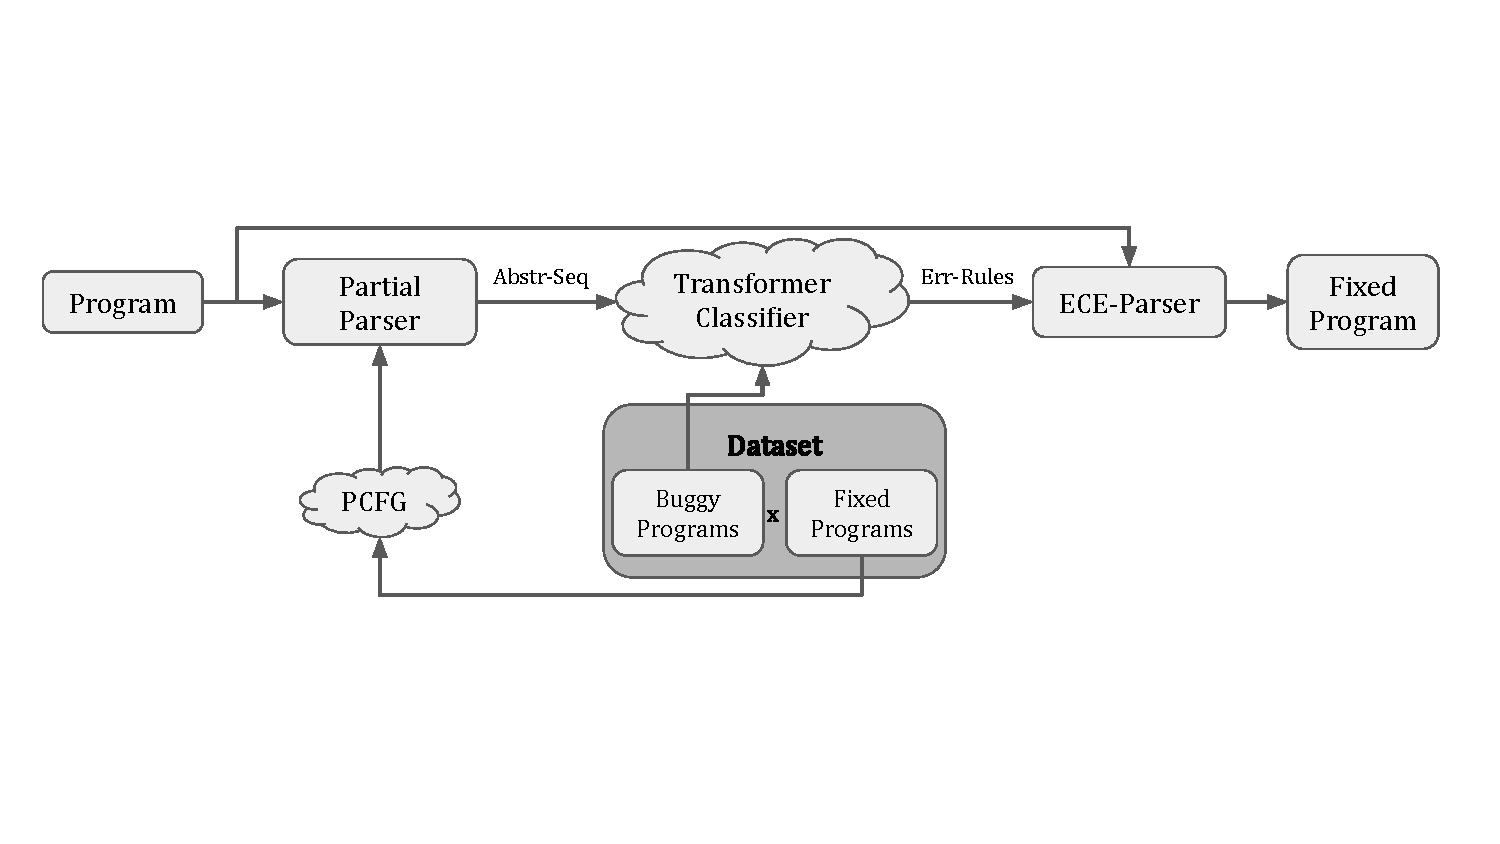
\includegraphics[trim={0 4.1cm 0 3.85cm}, clip, width=\linewidth]{overall-approach.pdf}
  \caption{\toolname's overall approach.}
  \label{fig:overall-approach}
\end{figure}

% \mypara{Error Correcting Parsers}
% One approach to fixing erroneous programs (as in \autoref{fig:bad-prog})
% is to use \emph{Error Correcting Parsers} (EC-Parsers) \citep{Aho_1972}.
% EC-Parsers are based on dynamic programming algorithms and have been used
% to automatically infer the intended parse trees for programs
% that have syntax errors. These dynamic programming parsers have been used
% with \emph{error correcting production rules} \citep{Aho_1972} to
% generate a valid parse by making minimal edits to the original program.
% However, EC-Parsers are very inefficient for larger
% grammars, since they require the addition of a large number of error production
% rules, making them impractical for real-world applications. In contrast, the
% original Earley parsing algorithm is also based on dynamic programming
% but does not directly support error correction~\citep{Earley_1970}.


\begin{figure}[t]
\begin{minipage}[c]{0.47\linewidth}
\begin{rules}
S        $\rightarrow$ Stmts end_marker
Stmts    $\rightarrow$ Stmt \n | Stmt \n Stmts
Stmt     $\rightarrow$ FuncDef | ExprStmt
          | RetStmt | PassStmt | ...
FuncDef  $\rightarrow$ def name Params : Block
Block    $\rightarrow$ \n indent Stmts dedent
RetStmt  $\rightarrow$ return | return Args
Args     $\rightarrow$ ExprStmt | ExprStmt , Args
ExprStmt $\rightarrow$ ArExpr | ...
ArExpr   $\rightarrow$ Literal
          | ArExpr BinOp Literal
Literal  $\rightarrow$ name | number | ...
\end{rules}
\caption{Simplified Python production rules.}
\label{fig:production-rules}
\end{minipage}
\hspace{0.02\linewidth}%
\begin{minipage}[c]{0.50\linewidth}
\hspace*{-0.06\linewidth}%
\begin{figure}
    \centering
    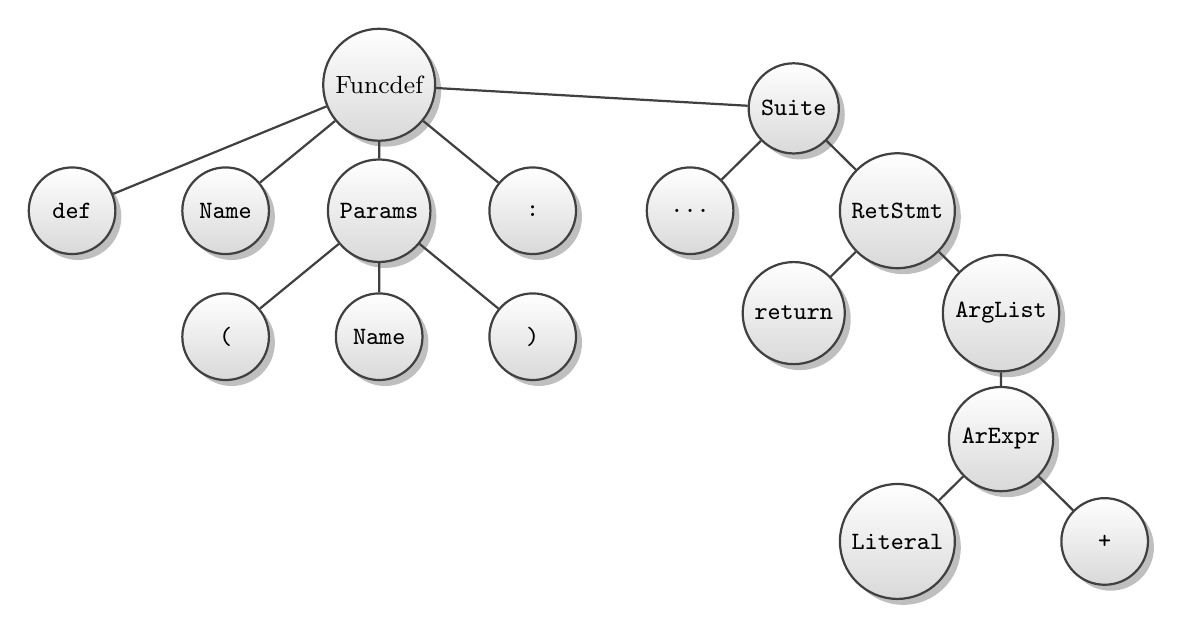
\begin{tikzpicture}
    [font=\small, edge from parent,
    every node/.style={top color=white, bottom color=black!15,
    circle, minimum size=11mm, draw=black!75,
    thick, drop shadow, align=center},
    edge from parent/.style={draw=black!75,thick},
    level distance=1.6cm, xscale=1.3]
    \node (func) {Funcdef}
        child {
            node (def) {\texttt{\bfseries def}}
        }
        child {
            node (name1) {\texttt{Name}}
        }
        child {
            node (params) {\texttt{Params}}
            child {
                node (openParen) {\texttt{\bfseries (}}
            }
            child {
                node (name2) {\texttt{Name}}
            }
            child {
                node (closeParen) {\texttt{\bfseries )}}
            }
        }
        child {
            node (colon) {\texttt{\bfseries :}}
        }
        child [level distance=0.3cm, xscale=1.35] {
            node  (suite) {\texttt{Suite}}
            child [level distance=1.3cm] {
                node (etc) {\texttt{...}}
            }
            child [level distance=1.3cm] {
                node (RetStmt) {\texttt{RetStmt}}
                % node (RetStmt) {\texttt{\begin{tabular}{c}
                %                                 Return\\
                %                                 Stmt
                %                             \end{tabular}}}
                child {
                    node (return) {\texttt{\bfseries return}}
                }
                child {
                    node (ArgList) {\texttt{ArgList}}
                    child [level distance=1.6cm] {
                        node (ArExpr1) {\texttt{ArExpr}}
                        child [level distance=1.3cm] {
                            node (ArExpr2) {\texttt{Literal}}
                        }
                        child [level distance=1.3cm] {
                            node (plus) {\texttt{\bfseries +}}
                        }
                    }
                }
            }
        };
    \end{tikzpicture}
    \caption{The partial parse tree generated for the example at \autoref{fig:orig-prog}}
    \label{fig:partial-parse-tree}
\end{figure}

\end{minipage}
\end{figure}

\subsection{Error-Correcting Parsing}
\label{sec:overview:ec-parsing}

\mypara{Earley Parsers for Python}
%
An Earley parser accepts programs that belong to a
language that is defined by a given \emph{grammar} $G$
by using dynamic programming, to store top-down partial
parses in a data structure called a \emph{chart} \citep{Earley_1970}.
The grammar $G$ has a starting symbol |S| and a set of \emph{production rules}.
\autoref{fig:production-rules} presents some simplified production rules for the
Python programming language that will help parse the program in
\autoref{fig:bad-prog}. \emph{Terminal} symbols (or \emph{tokens}) are
syntactical symbols and are here presented in lowercase
letters. Uppercase letters denote \emph{non-terminal} symbols, which are
rewritten using production rules during a parse.
For example, the non-terminal |Stmt| defines all
possible Python statements, including expressions (|ExprStmt|), return statements
(|RetStmt|), \etc \autoref{fig:partial-parse-tree-1} shows the top levels of
the parse tree for the |bar| function in \autoref{fig:bad-prog} using these
productions rules.

%
% \begin{figure}[t]
% \begin{ecode}
% New_S     (*@$$\rightarrow$@*) S | S Insert
% ...
% Block     (*@$$\rightarrow$@*) E_\n E_indent Stmts E_dedent
% RetStmt   (*@$$\rightarrow$@*) ... | E_return | E_return Args
% ...
% E_return  (*@$$\rightarrow$@*) return | (*@$\epsilon$@*) | Replace | Insert return
% E_number  (*@$$\rightarrow$@*) number | (*@$\epsilon$@*) | Replace | Insert number
% E_\n      (*@$$\rightarrow$@*) \n | (*@$\epsilon$@*) | Replace | Insert \n
% ...
% Replace   (*@$$\rightarrow$@*) return | pass | \n | ... [all terminals]
% Insert    (*@$$\rightarrow$@*) Token | Insert Token
% Token     (*@$$\rightarrow$@*) return | pass | \n | ... [all terminals]
% \end{ecode}
% \caption{Error production rules for the simplified Python grammar presented in
% \autoref{fig:production-rules}}
% \label{fig:error-rules}
% \end{figure}

\mypara{Error-Correcting Parsers for Python}
%
An \emph{Error-Correcting Earley} (ECE) Parser
extends the original algorithm's operations,
to find a \emph{minimum-edit} parse for a program
with parse errors~\citep{Aho_1972}.
%
An ECE-Parser extends the original grammar $G$
with a set of \emph{error production rules} to
create a new \emph{error grammar} $G'$ which has
rules to handle \emph{insertion}, \emph{deletion},
and \emph{replacement} errors.
%
Let's see how to adapt Python's
production rules for an ECE-Parser.
%
First, the ECE-Parser adds to $G'$ a new start symbol |New_S|, the helper
symbol |Replace| that is used for replacement errors and the symbols |Insert|
and |Token| that introduce insertion errors. Additionally, for each terminal |t|
in $G$ it adds the new non-terminal |E_t| that introduces errors relevant to the
|t| symbol.

Next, in addition to the existing production rules, the error grammar $G'$ has
the following error rules. The new start symbol uses the old one with the option
of an insertion error at the end:
\begin{itemize}
  \item \lstinline{New_S  $\rightarrow$ S | S Insert}
\end{itemize}
Additionally, for each production rule of a non-terminal |T| in $G$, another
non-terminal error rule is added that introduces the terminal symbols |E_t|, for
each original terminal |t| it has. For example, the |Stmts|, |Block| and
|RetStmt| rules are updated as:
\begin{itemize}
  \item \lstinline{Stmts    $\rightarrow$ ... | Stmt E_\n | Stmt E_\n Stmts}
  \item \lstinline{Block    $\rightarrow$ ... | E_\n E_indent Stmts E_dedent}
  \item \lstinline{RetStmt  $\rightarrow$ ... | E_return | E_return Args}
\end{itemize}
Next, for each terminal |t| in $G$, we add four error rules of the type:
\begin{itemize}
  \item \lstinline{E_t $\rightarrow$ t | $\epsilon$ | Replace | Insert t}
\end{itemize}
These four new error rules have the following usage for each terminal |t|:
\begin{enumerate}
  \item The |E_t $\rightarrow$ t| rule will match the original terminal |t|
  without any errors. This error rule is used in cases that the \emph{non-error}
  version of the rule is needed. For example, in |Block $\rightarrow$| \break
  |E_\n E_indent Stmts E_dedent| it can be the case that only
  |E_dedent| is needed to match the error and |E_\n| and |E_indent| can match
  their respective symbols.
  \item Using |E_t $\rightarrow$ $\epsilon$| a \emph{deletion} error is
  considered. The error rule will match \emph{nothing}, or the \emph{empty
  token} $\epsilon$, in the program, meaning the terminal is missing.
  \item Using |E_t $\rightarrow$ Replace| a \emph{replacement} error is considered.
  |Replace| will match any terminal token that is \emph{different} than |t|,
  making a replacement possible.
  \item  The rules |E_t $\rightarrow$ Insert t| will introduce an
  \emph{insertion} error, \ie |Insert| will match any \emph{sequence} of
  |Token|s that are not supposed to precede |t| in order to make the program
  parse.
\end{enumerate}
% When, for example, a \texttt{Return\_Stmt} is added to the ECE-Parser's chart at
% some location $i$, then the next four options are considered:
% \begin{enumerate}
%   \item There is a \texttt{\bfseries return} at location $i+1$ of the tokenized
%   program and therefore the original \emph{non-error} production rules are used
%   to and are added to the chart at location $i+1$.
%   \item An \emph{insertion} error is considered, \ie there is a token at program
%   location $i$ that doesn't match any of the production rules. Then
%   \texttt{Err\_Return $\rightarrow$ H return} is used to introduce one or more of these
%   insertion errors together with the rules \texttt{H $\rightarrow$ H \textbar\ H Insert}
%   and \texttt{Insert $\rightarrow$ \textbf{pass} \textbar\ \textbf{raise} \textbar\
%   \textbf{return} \textbar\ ...}. When \texttt{Insert} will match an
%   extraneous token $t$ in the program, then $t$ will be ignored in the final
%   parse repair.
%   \item A \emph{deletion} error is considered when an incomplete non-terminal
%   production rule is in the chart at location $i$ and the next symbol is a
%   terminal in the rule but is not present in the token sequence. Then
%   \texttt{Err\_Return $\rightarrow$ e} is used to match an \emph{empty} token. At the final
%   stage, the relevant terminal (here a \texttt{\textbf{return}}) will be added
%   at location $i+1$ to generate a repaired program.
%   \item A \emph{replacement} error is considered here when an incomplete
%   non-terminal production rule is in the chart at location $i$ and the next
%   symbol is a terminal in the rule but is not the same in the token sequence.
%   Then \texttt{Err\_Return $\rightarrow$ Err\_Tag} is used to match the program token $t$.
%   At the final stage, the relevant terminal (here a \texttt{\textbf{return}})
%   will replace the program token $t$.
% \end{enumerate}

For example, for the terminal tokens |return|, |number| and |\n| (a new line)
the relevant error production rules are:
\begin{itemize}
  \item \lstinline{E_return  $\rightarrow$ return | $\epsilon$ | Replace | Insert return}
  \item \lstinline{E_number  $\rightarrow$ number | $\epsilon$ | Replace | Insert number}
  \item \lstinline{E_\n      $\rightarrow$ \n | $\epsilon$ | Replace | Insert \n}
\end{itemize}
Finally, the |Replace| non-terminal can match any possible terminal in $G$ to
introduce replacement errors, the |Insert| non-terminal will introduce a
sequence of insertion errors by using |Token| which also matches every terminal
and we just differentiate the name in order to be able to distinguish the
different types of errors.
\begin{itemize}
  \item \lstinline{Replace  $\rightarrow$ return | pass | \n | + | ... [all terminals]}
  \item \lstinline{Insert   $\rightarrow$ Token | Insert Token}
  \item \lstinline{Token    $\rightarrow$ return | pass | \n | + | ... [all terminals]}
\end{itemize}

\begin{figure}
    \centering
    \begin{minipage}[t]{0.28\linewidth}
        \centering
        \resizebox{!}{0.25\textheight}{
        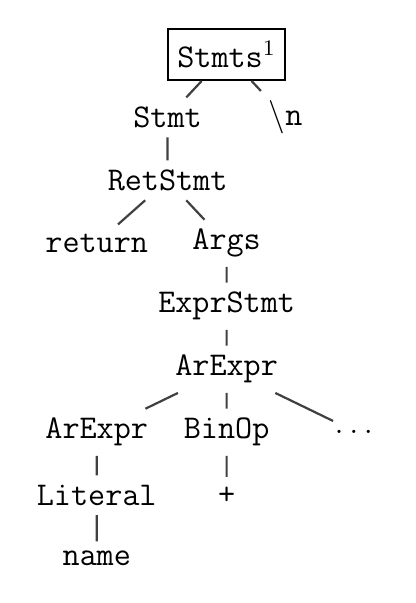
\begin{tikzpicture}
        [font=\large, edge from parent,
        % every node/.style={top color=white, bottom color=black!20,
        % ellipse, minimum size=8mm, draw=black!75,
        % thick, drop shadow, align=center},
        edge from parent/.style={draw=black!75, thick},
        level distance=0.8cm, xscale=1.0]
        \node [style={minimum size=6.5mm, draw=black, thick}] (stmts2) {\texttt{Stmts$^1$}}
        child {
            node (stmt2) {\texttt{Stmt}}
            child {
                node (RetStmt) {\texttt{RetStmt}}
                child [xscale=1.2] {
                    node (return) {\texttt{\bfseries return}}
                }
                child {
                    node (args) {\texttt{Args}}
                    child {
                        node (expr2) {\texttt{ExprStmt}}
                        child [xscale=1.1] {
                            node (arexpr1) {\texttt{ArExpr}}
                            child {
                                node (arexpr2) {\texttt{ArExpr}}
                                child {
                                    node (literal) {\texttt{Literal}}
                                    child {
                                        node (name3) {\texttt{name}}
                                    }
                                }
                            }
                            child {
                                node (binop) {\texttt{BinOp}}
                                child {
                                    node (plus) {\texttt{\bfseries +}}
                                }
                            }
                            child {
                                node (empty) {\texttt{$\dots$}}
                            }
                        }
                    }
                }
            }
        }
        child {
            node (newline3) {\texttt{\textbackslash n}}
        };
        \end{tikzpicture}
        } \subcaption{The partial parse tree for the example at
        \autoref{fig:bad-prog}.}
        \label{fig:partial-parse-tree-2}
    \end{minipage}
    \hspace{0.02\linewidth}%
    \begin{minipage}[t]{0.35\linewidth}
        \centering
        \hspace*{0.04\linewidth}%
        \resizebox{!}{0.25\textheight}{
            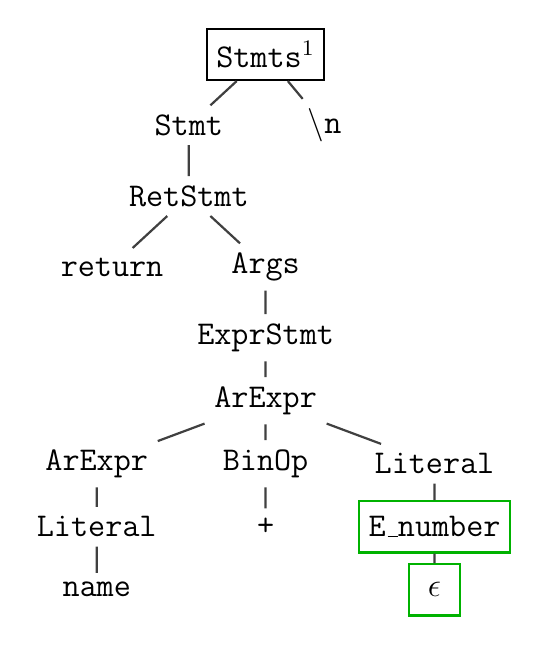
\begin{tikzpicture}
            [font=\large, edge from parent,
            % every node/.style={top color=white, bottom color=black!20,
            % ellipse, minimum size=8mm, draw=black!75,
            % thick, drop shadow, align=center},
            edge from parent/.style={draw=black!75, thick},
            level distance=0.9cm, xscale=1.0]
            \node [style={minimum size=6.5mm, draw=black, thick}] (stmts2) {\texttt{Stmts$^1$}}
            child [xscale=1.3] {
                node (stmt2) {\texttt{Stmt}}
                child {
                    node (RetStmt) {\texttt{RetStmt}}
                    child {
                        node (return) {\texttt{\bfseries return}}
                    }
                    child {
                        node (args) {\texttt{Args}}
                        child {
                            node (expr2) {\texttt{ExprStmt}}
                            child [level distance=0.8cm, xscale=1.1] {
                                node (arexpr1) {\texttt{ArExpr}}
                                child {
                                    node (arexpr2) {\texttt{ArExpr}}
                                    child {
                                        node (literal1) {\texttt{Literal}}
                                        child {
                                            node (name3) {\texttt{name}}
                                        }
                                    }
                                }
                                child {
                                    node (binop) {\texttt{BinOp}}
                                    child {
                                        node (plus) {\texttt{\bfseries +}}
                                        }
                                }
                                child {
                                    node (literal2) {\texttt{Literal}}
                                    child {
                                        node [style={minimum size=6.5mm, draw=black!30!green, thick}] (enumber) {\texttt{E\_number}}
                                        child {
                                            node [style={minimum size=6.5mm, draw=black!30!green, thick}] (eps) {\texttt{$\epsilon$}}
                                        }
                                    }
                                }
                            }
                        }
                    }
                }
            }
            child {
                node (newline3) {\texttt{\textbackslash n}}
            };
            \end{tikzpicture}
        } \subcaption{Adding a number with the green \texttt{E\_number} error rule.}
        \label{fig:adding-partial}
    \end{minipage}
    \hspace{0.01\linewidth}%
    \begin{minipage}[t]{0.32\linewidth}
        \centering
        \resizebox{!}{0.25\textheight}{
            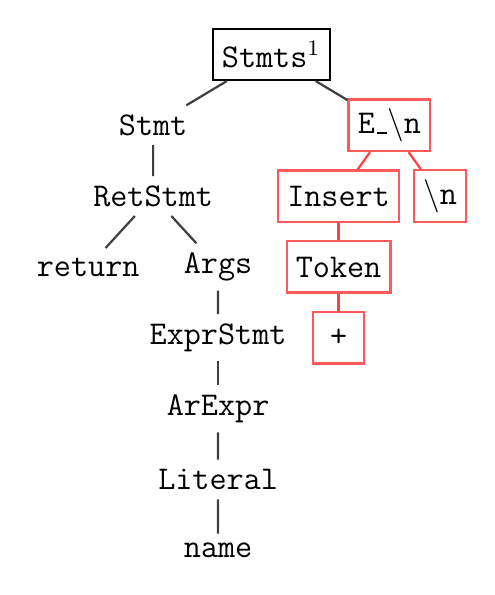
\begin{tikzpicture}
            [font=\large, edge from parent,
            % every node/.style={top color=white, bottom color=black!20,
            % ellipse, minimum size=8mm, draw=black!75,
            % thick, drop shadow, align=center},
            edge from parent/.style={draw=black!75, thick},
            level distance=0.9cm, xscale=2.0]
            \node [style={minimum size=6.5mm, draw=black, thick}] (stmts2) {\texttt{Stmts$^1$}}
            child {
                node (stmt2) {\texttt{Stmt}}
                child [xscale=0.55] {
                    node (RetStmt) {\texttt{RetStmt}}
                    child {
                        node (return) {\texttt{\bfseries return}}
                    }
                    child {
                        node (args) {\texttt{Args}}
                        child {
                            node (expr2) {\texttt{ExprStmt}}
                            child {
                            node (arexpr1) {\texttt{ArExpr}}
                                child {
                                    node (literal1) {\texttt{Literal}}
                                    child {
                                        node (name3) {\texttt{name}}
                                    }
                                }
                            }
                        }
                    }
                }
            }
            child {
                node [style={minimum size=6.5mm, draw=red!65, thick}] (enewline) {\texttt{E\_\textbackslash n}}
                child [edge from parent/.style={draw=red!75, thick}, xscale=0.43] {
                    node [style={minimum size=6.5mm, draw=red!65, thick}] (insert) {\texttt{Insert}}
                    child {
                        node [style={minimum size=6.5mm, draw=red!65, thick}] (token) {\texttt{Token}}
                        child {
                            node [style={minimum size=6.5mm, draw=red!65, thick}] (plus) {\texttt{\bfseries +}}
                        }
                    }
                }
                child [edge from parent/.style={draw=red!75, thick}, xscale=0.43] {
                    node [style={minimum size=6.5mm, draw=red!65, thick}] (newline3) {\texttt{\textbackslash n}}
                }
            };
            \end{tikzpicture}
        }
        \subcaption{Deleting the \texttt{+} with red \texttt{E\_\textbackslash n} error rule.}
        \label{fig:deleting-partial}
    \end{minipage}
    \caption{The rest of the problematic function in
    \autoref{fig:partial-parse-tree-1} and two possible error-correcting parses}
    \label{fig:two-partial-parses}
\end{figure}




% This eliminates backtracking and prevents a combinatorial explosion. Worst
% case, it has a time complexity of $O(n^3 G^2)$ for generic context-free
% grammars, where $n$ is the number of \emph{tokens} of the input program and
% $G$ is the grammar size, \ie the number of \emph{production rules} it
% includes.

% Therefore, the new and larger error correcting grammar $G'$ is introduced that
% is at least 3 times larger than $G$, making ECE-Parser not scalable for large
% programs or programs with a lot of parse errors.

\mypara{ECE Parsing Considerations for Python}
%
Unfortunately, we run into various problems if we
try to directly use an ECE-Parser for large, real-world
languages like Python.
%
\autoref{fig:partial-parse-tree-2} presents a \emph{partial
parse} of the problematic statements |Stmts|$^1$ of
\autoref{fig:partial-parse-tree-1}.
%
Considering a deletion error (\autoref{fig:adding-partial}), the
%
|E_number $\rightarrow$ $\epsilon$| error rule is used to match the empty symbol
and generate a parse that suggests that a \emph{number} is missing after the |+|
operator. On the other hand, the
%
|E_\n $\rightarrow$ Insert \n| error rule can be used to consider an insertion
error (\autoref{fig:deleting-partial}) before the new line character, basically
\emph{deleting} the |+| operator. In this case, |ArExpr $\rightarrow$ Literal|
is used to parse the program instead of
%
|ArExpr $\rightarrow$ ArExpr BinOp Literal|.

The ECE-Parser is an effective approach on finding minimum distance parses for
programs than do not belong in the given programming language, \ie have parse
errors. However, this parsing algorithm has limited use in large real-world
programming languages, \eg Python or Java, and more time- and memory-efficient
parsing algorithms are often used, \eg LR parsing \etc \citep{Knuth_1965,
Chapman_1987}. For example, Python has \emph{$91$ terminal symbols} (including
the program's |end_marker|) which means that for all the cases of the error
rules |E_t| (excluding the non-error base case |E_t $\rightarrow$ t|), |Replace|
and |Token|, \emph{$455$ terminal error rules} have to be added to the grammar
$G'$. The Python grammar that we used has also \emph{$283$ production rules},
from which \emph{$182$ rules} have terminals in them, meaning another
\emph{$182$ error rules} need to be added. Including the four helper production
rules, \eg for the new start symbol, the new grammar $G'$ has \emph{$641$ new
error production rules}. This large amount of error rules renders the ECE-Parser
not scalable for large programs or programs with a lot of parse errors when
using real-world programming languages.

One of our insights,
as seen in our running example in \autoref{fig:two-partial-parses}, is that only
a handful of error rules are relevant to each parse error. Therefore, we
propose to improve ECE-Parsing's scalability by only adding \emph{a
small set} of error production rules, \ie keeping the size of $G'$ limited and
only slightly larger than the original grammar $G$. We propose to do so by
\emph{training classifiers} to select a small set of error rules only relevant
to the parse error. However, the program token sequences that we can use
may have irrelevant information, \eg the |foo| function in our example in
\autoref{fig:example-prog} that does not contribute to the parse error. To
address this problem, we propose to further \emph{abstract} our program token
sequences.

\subsection{Abstracting Program Token Sequences}
\label{sec:overview:abstraction}

As shown in \autoref{fig:overall-approach}, our neural component has the task of
training a classifier to predict the relevant error rules for a given ill-parsed
program.

\mypara{Problem: Representing Ill-parsed Programs}
%
As the inputs are ill-parsed, the training and classification
cannot use any form of analysis that requires a syntax tree as
input \citep{Sakkas_2020, Martinez_2013, Gulwani_2018, Wang_2018}.
%
One option is to view the ill-parsed program as a
plain \emph{sequence of tokens} eliding variable
names and such, as shown in \autoref{fig:prog-seq}.
%
Unfortunately, we found such token sequences yielded inaccurate classifiers that
were confused by irrelevant trailing context and predicted rules that were not
relevant to repair the error at hand.


\begin{figure}[t]
\centering
\begin{minipage}[t]{0.56\linewidth}
\centering
\begin{ecode}
def name(name): \n
indent return name + number \n
dedent \n

def name(name): \n
indent name = name(name) + number \n
return name + \n
dedent end_marker
\end{ecode}
\subcaption{The token sequence generated by the lexer for the program.}
\label{fig:prog-seq}
\end{minipage}%
\hspace{0.02\linewidth}%
\begin{minipage}[t]{0.42\linewidth}
\centering
\begin{ecode}
Stmt \n

def name Params: \n
indent Stmt \n
return Expr BinOp \n
dedent end_marker
\end{ecode}
\subcaption{The abstracted token sequence for the same program.}
\label{fig:abstract-prog-seq}
\end{minipage}
\caption{The token sequences for the Python program example in \autoref{fig:example-prog}.}
\end{figure}

\mypara{Solution: Abstract with Partial Parses}
%
\toolname solves the problem of irrelevant context by \emph{abstracting} the
token sequences using \emph{partial parses} to abstract away the irrelevant
context.
%
That is, we can use partial parse trees to represent ill-parsed programs as an
\emph{abstracted token sequence} shown in \autoref{fig:abstract-prog-seq}, where
any \emph{completed} production rules can be used to abstract the relevant
\emph{token sub-sequences} with the high-level \emph{non-terminal}.

\autoref{fig:partial-parse-tree-1} shows how partial parses can be used to
abstract long low-level sequences of tokens into short sequences of
non-terminals.
%
(1)~The function |foo| is completely parsed,
since it had no parse errors and the highest
level rule that can be used to abstract it is
%
|Stmt $\rightarrow$ FuncDef|.
%
(2)~Similarly, note that |Params $\rightarrow$ ( name )|
is another completed production rule, therefore the
low-level sequence of  parameter tokens in the |bar|
function can be abstracted to just the non-terminal |Params|.
%
(3)~However, the production rule for |FuncDef| is \emph{incomplete} since the
last statement |Stmt| (under |Stmts|$^1$) has a parse error as shown in
\autoref{fig:partial-parse-tree-2}.

\mypara{Problem: Ambiguity}
%
The generation of this abstraction, however,
poses another difficulty.
%
Earley parsing collects a large amount of partial
parses (via dynamic programming) until the program
is fully parsed.
%
That means at each program location, multiple
partial parses can be chosen to abstract our programs.
%
This \emph{ambiguity} can be seen even in the two
suggested repairs in \autoref{fig:two-partial-parses}:
if we delete the colored nodes in \autoref{fig:adding-partial} and
\autoref{fig:deleting-partial} we obtain two possible partial parses for our
program, the first one matching \autoref{fig:partial-parse-tree-2} and the
second one not shown here.

\mypara{Solution: Probabilistic Context-Free Grammars}
%
\toolname solves the ambiguity problem
of choosing between multiple possible
partial parses via a data-driven approach
based on \emph{Probabilistic Context-Free Grammars}
which have been used in previous work
to select \emph{complete} parses for
ambiguous grammars \citep{Collins_2013, Jelinek_1992}.
%
A PCFG associates each of its production rules with a
\emph{weight} or \emph{probability}.
%
These weights can be learned \citep{Collins_2013}
by using the data set to count the production rules
used to parse a number of programs belonging to that
language.
%
\toolname uses PCFGs to resolve the ambiguity of
partial parses by associating each partial tree
(in the Earley table) with a probability which
is the \emph{product} of the used rules' probabilities.
%
The tree with the highest probability is selected
as a final parse tree which can then be used to
generate an abstracted token sequence, as described above.


\autoref{fig:weighted-production-rules} shows the
learned probabilities for the example Python grammar.
%
We observe, for example, that |ReturnStmt| has two
possible production rules and almost $98.4\%$ of the
times a |return| is followed by an argument list.
%
Additionally, $62.6\%$ of the times a |Stmt| is an
|ExprStmt| and only $7.6\%$ of the times it is a |RetStmt|.
%
Thus, in our example, the probability that would be assigned
to the partial parse for |Stmts|$^1$ in \autoref{fig:adding-partial}
(only the sub-tree without the colored error nodes) is
the product of the probabilities of the production rules |Stmts|
$\rightarrow$ |Stmt \n|, |Stmt| $\rightarrow$ |RetStmt|, |RetStmt| $\rightarrow$
|return Args|, |Args| $\rightarrow$ |ExprStmt| \etc which is $38.77\%\ \cdot\
7.59\%\ \cdot\ 98.39\%\ \cdot\ 99.20\%\ \cdot\ \dots =
4.57\text{\textperthousand}$, while the partial parse for |Stmts|$^1$ in
\autoref{fig:deleting-partial} would similarly be calculated as
$47.61\text{\textperthousand}$, making it the proper choice for
the abstraction of the program.

\begin{figure}[t]
\begin{rules}
S        $\rightarrow$ Stmts end_marker ($p = \underline{100.0\%}$)
Stmts    $\rightarrow$ Stmt \n ($p = \underline{38.77\%}$) | Stmt \n Stmts ($p = \underline{61.23\%}$)
Stmt     $\rightarrow$ ExprStmt ($p = \underline{62.64\%}$) | RetStmt ($p = \underline{ 7.59\%}$) | ...
RetStmt  $\rightarrow$ return ($p = \underline{ 1.61\%}$) | return Args ($p = \underline{98.39\%}$)
Args     $\rightarrow$ ExprStmt ($p = \underline{99.20\%}$) | ...
ExprStmt $\rightarrow$ ArExpr ($p = \underline{29.40\%}$) | ...
ArExpr   $\rightarrow$ Literal ($p = \underline{86.89\%}$) | ArExpr BinOp Literal ($p = \underline{13.11\%}$)
Literal  $\rightarrow$ name ($p = \underline{64.89\%}$) | number ($p = \underline{20.17\%}$) | ...
\end{rules}
\caption{The production rules shown in \autoref{fig:production-rules} with
their learned \underline{probabilities}.}
\label{fig:weighted-production-rules}
\end{figure}
% S        (*@$\rightarrow$@*) Stmts end_marker        , $p = 100.0\%$
% Stmts    (*@$\rightarrow$@*) Stmt \n                 , $p = 38.77\%$
% Stmt     (*@$\rightarrow$@*) ExprStmt                , $p = 62.64\%$
% Stmt     (*@$\rightarrow$@*) RetStmt                 , $p =  7.59\%$
% RetStmt  (*@$\rightarrow$@*) return                  , $p =  1.61\%$
% RetStmt  (*@$\rightarrow$@*) return Args             , $p = 98.39\%$
% Args     (*@$\rightarrow$@*) ExprStmt                , $p = 99.20\%$
% ExprStmt (*@$\rightarrow$@*) ArExpr                  , $p = 29.40\%$
% ArExpr   (*@$\rightarrow$@*) Literal                 , $p = 86.89\%$
% ArExpr   (*@$\rightarrow$@*) ArExpr BinOp Literal    , $p = 13.11\%$
% Literal  (*@$\rightarrow$@*) name                    , $p = 64.89\%$
% Literal  (*@$\rightarrow$@*) number                  , $p = 20.17\%$
% Stmts    (*@$\rightarrow$@*) Stmt \n Stmts           , $p = 61.23\%$
% Stmt     (*@$\rightarrow$@*) FuncDef                 , $p =  7.86\%$
% Stmt     (*@$\rightarrow$@*) PassStmt                , $p =  0.13\%$
% FuncDef  (*@$\rightarrow$@*) def name Params : Block , $p = 99.10\%$
% Block    (*@$\rightarrow$@*) \n indent Stmts dedent  , $p = 99.29\%$
% Args     (*@$\rightarrow$@*) ExprStmt , Args         , $p =  0.80\%$

\subsection{Training Sequence Classifiers}
\label{sec:overview:train}

The abstracted token sequences we extracted from
the partial parses present us with short abstracted
sequences that abstract irrelevant details of the context
into non-terminals.
%
Next, \toolname uses the NLP approach of \emph{sequence models}
\citep{Sutskever_2014, Hardalov_2018} to (use the abstract token sequences) to
train a classifier that can predict the relevant error rules.

\mypara{Seq2Seq Architectures}
%
Sequence-to-sequence (seq2seq) architectures
transform an input sequence of tokens into a
new sequence \citep{Sutskever_2014} and consist
of an \emph{encoder} and a \emph{decoder}.
%
The encoder transforms the input sequence into an \emph{abstract vector} that
captures all the essence and context of the input.
%
This vector does not necessarily have a physical
meaning and is instead an internal representation
of the input sequence into a higher dimensional space.
The abstract vector is given as an input to the decoder,
which in turn transforms it into an output sequence.

% Both the encoder and the decoder can be an (older) Long-Short-Term-Memory
% (LSTM)-based model \citep{Hochreiter_1997} or a more modern and state-of-the-art
% \emph{Transformer} \citep{Vaswani_2017}.

\toolname uses a \emph{sequence classifier} that can correctly predict a small
set of relevant error production rules for a given abstracted token sequence. We
use a \emph{transformer encoder} \citep{Vaswani_2017} to encode the input
sequences into abstract vectors that we then feed into a \emph{\dnn} classifier
to train and make accurate predictions \citep{Schmidhuber_2015}.

\mypara{Training From a Dataset}
%
Given a dataset of fixed parse errors,
such as \autoref{fig:example-prog}, we
extract the small set of relevant error
rules needed for each program to make it parse
with an ECE-Parser.
%
Running the ECE-Parser on every program
in the dataset with the \emph{full set}
of error production rules is prohibitively
slow.
%
Therefore, we extract the erroneous and
fixed program token-level differences or
\emph{token diffs} and map them to
\emph{terminal error production rules}.
%
The non-terminal error rules can be
inferred using the grammar and the terminal
rules. Next, we run the ECE-Parser with
the extracted error rules to confirm which
ones would make the program parse and assign them as
\emph{labels}.

For example, the diff for the program pair in
\autoref{fig:example-prog} would show the
deleted |+| operator, thus extracting
the error rules |Token $\rightarrow$ +|
and |E_\n $\rightarrow$ Insert \n|,
since the extra |+| precedes
a newline character |\n|.
%
Similarly, if a token |t| is added in
the fixed program, the error rule
%
|E_t $\rightarrow$ $\epsilon$| is added and if a token |t| replaces a token |a|,
the error rules |E_t $\rightarrow$ Replace| and
%
|Replace $\rightarrow$ a| are added.

\subsection{Predicting Error Rules with Sequence Classifiers}
\label{sec:overview:seq-classifiers}

The learned sequence classifier model, which has been trained on the updated
error-rule-labeled data set can now be used to predict the relevant rules for
new erroneous programs.
%
Additionally, neural networks have
the advantage of associating each
class with a \emph{confidence score}
that can be used to rank error rule
predictions for new programs, letting
us select the top-$N$ ones that will
yield accurate repairs when used
with the ECE-Parser.

For our running example, in \autoref{fig:bad-prog}, we abstract the program as
shown in \autoref{fig:abstract-prog-seq} and then we predict the error
production rules for it with the trained sequence classifier. We rank the full
set of \emph{terminal} error rules based on their predicted confidence score
from the classifier and return the \emph{top 10} predictions for our example.
Therefore, the predicted set of error rules is the following:
%
|E_number $\rightarrow$ $\epsilon$|,
%
|E_number $\rightarrow$ Insert number|, |E_\n $\rightarrow$ Insert \n|,
%
|E_($\rightarrow$ $\epsilon$|,
%
|E_return $\rightarrow$ $\epsilon$|, |Token $\rightarrow$ )|,
%
|Token $\rightarrow$ +|, |Token $\rightarrow$ :|, |Token $\rightarrow$ name|,
%
|Token $\rightarrow$ number|.

The classifier predicts mostly relevant error rules such as the ones that use
|E_number|, |E_\n| and |E_return| for example, as we showed previously. There
are also rules that are not very relevant to this parse error but the classifier
predicts probably due to them being common parse errors, \eg
%
|Token $\rightarrow$ )|, |Token $\rightarrow$ :|. Finally, we added the
\emph{non-terminal} error rules needed to introduce these errors, which can be
inferred by them. For example, we can infer
%
|Stmts $\rightarrow$ Stmt E_\n|, |Stmts $\rightarrow$ Stmt E_\n Stmts| and
%
\lstinline{Block $\rightarrow$ E_\n indent Stmts dedent} from |E_\n| (we don't
need \linebreak |E_indent| or |E_dedent| here since no such terminal error rules were
predicted).

We then parse the program in \autoref{fig:bad-prog} with the ECE-Parser and
these specific error rules to generate a valid parse. We observe that it takes
our implementation (as we show later in depth) less than \emph{2 seconds} to
generate a valid parse, which is also the one that leads to the user repair in
\autoref{fig:fixed-prog}! On the other hand, when we use a baseline ECE-Parser
with the full set of error rules it takes \emph{2 minutes and 55 seconds} to
generate a valid parse, which is, however, not the expected user parse but the
one shown in \autoref{fig:adding-partial}. These examples demonstrate the
effectiveness of accurately \emph{predicting error rules using sequence
classifiers, which are trained on abstracted token sequences}.

In the next three sections, we describe in depth the specifics of our approach
by defining all the methods in \autoref{fig:api}. We start by presenting the
program abstraction (\autoref{sec:prog-abstract}) using partial parses and a
learnt PCFG, we then explain how we train sequence models for making error rule
predictions (\autoref{sec:seq-classifiers}) and, finally, we demonstrate our
algorithms for building \toolname (\autoref{sec:whole-system}), an approach for
efficiently parsing erroneous programs.

\section{A Case for Parse Error Repair}
\label{sec:error-analysis}

We motivate \toolname by analyzing a dataset
comprising \emph{1,100,000 erroneous Python programs}
and their respective fixes.
%
This dataset was gathered from PythonTutor.com~\citep{Guo2013}
between the years 2017 and 2018, previously used in related
work~\citep{Endres2019, Cosman2020}.
%
Each program which throws an uncaught \python exception
is paired with the next program by the same user that does
not crash, under the assumption that the latter is the fixed
version of the former.
%
We discard pairs that are too different between buggy
and fixed versions, since these are usually unrelated
submissions or complete refactorings.
%
We also discard submissions that violate PythonTutor's
policies (\eg, those using forbidden libraries).
%
The resulting dataset contains usable program pairs,
representing students from dozens of universities
(PythonTutor has been used in many introductory
courses~\citep{Guo2013}) as well as non-traditional
novices.

\begin{figure}[t]
  \centering
  \begin{minipage}[c]{0.48\linewidth}
    \centering
    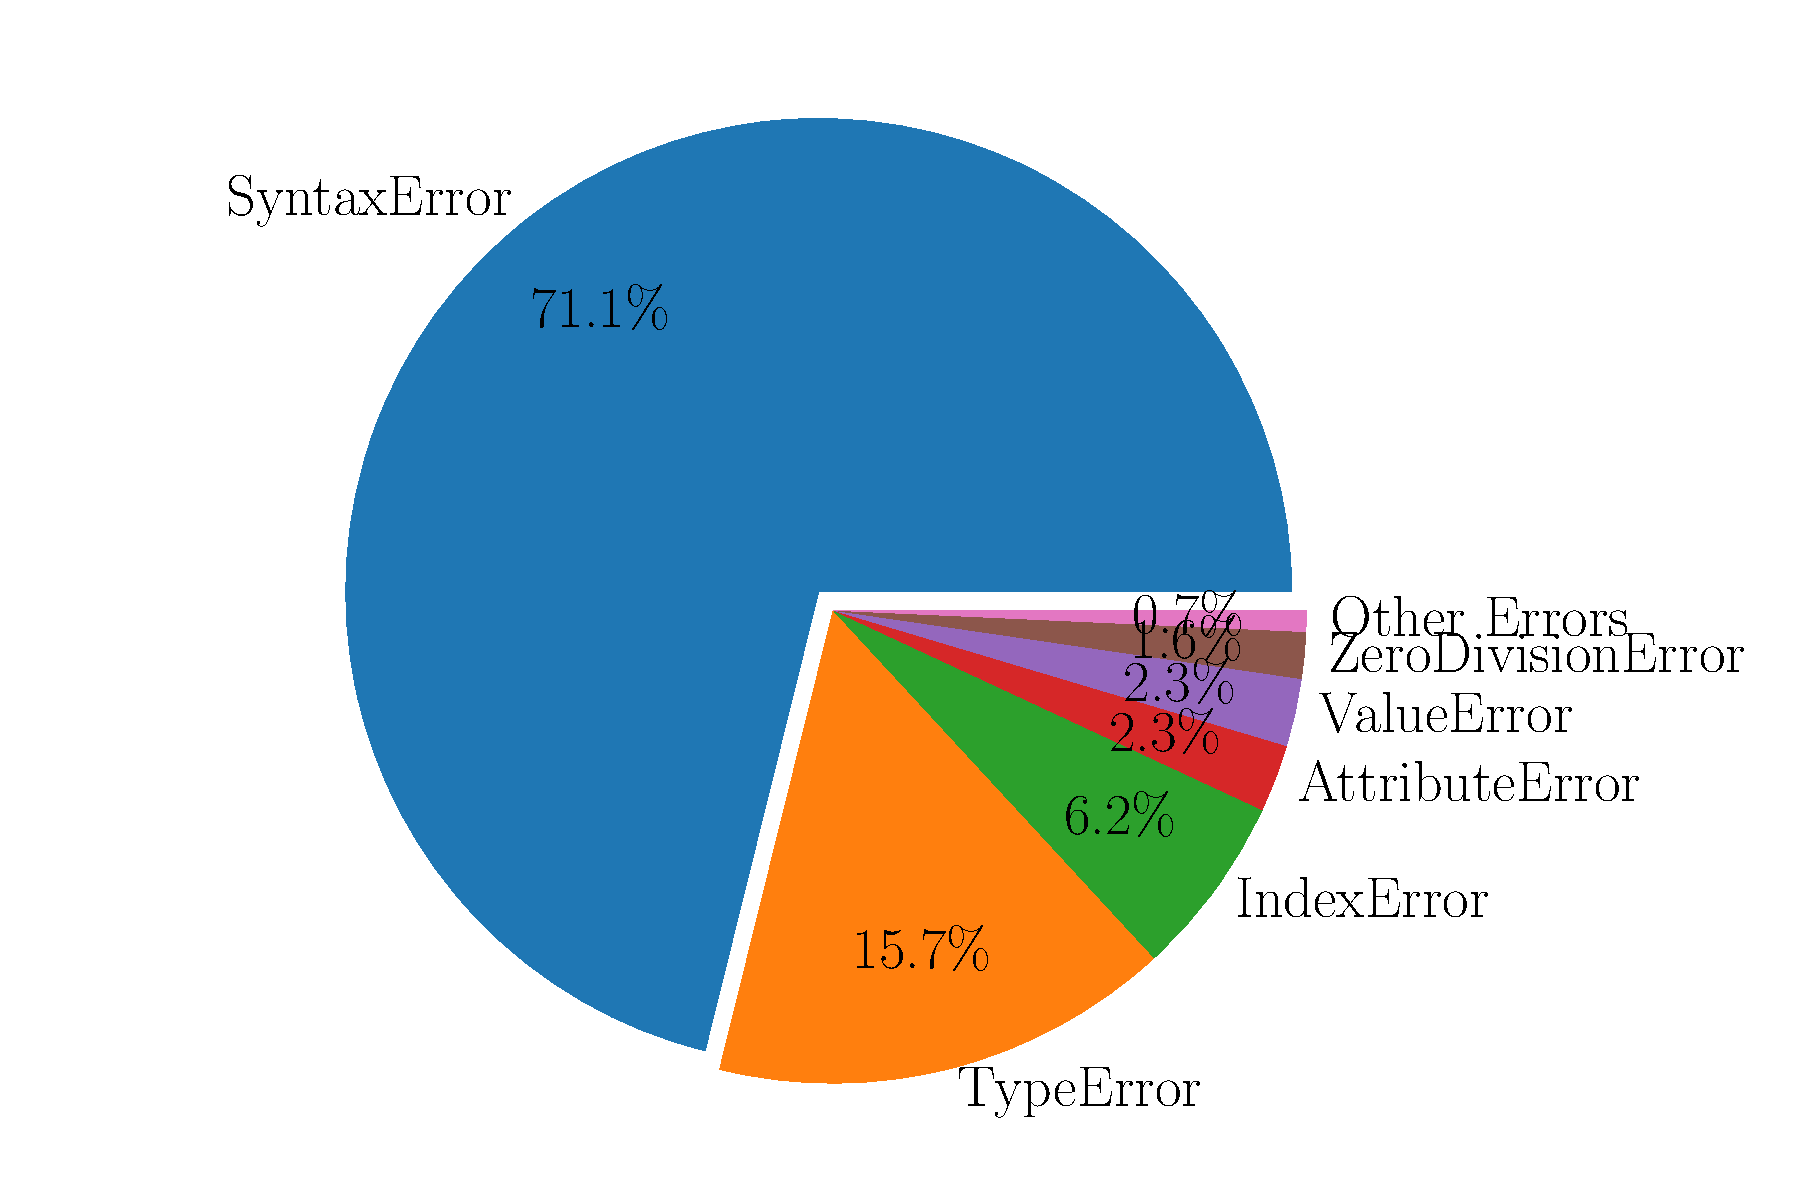
\includegraphics[width=\linewidth]{error-pie.pdf}
    \caption{The Python error type distribution.}
    \label{fig:error-statistics}
  \end{minipage}
  \hspace{0.02\linewidth}
  \begin{minipage}[c]{0.48\linewidth}
      \centering
      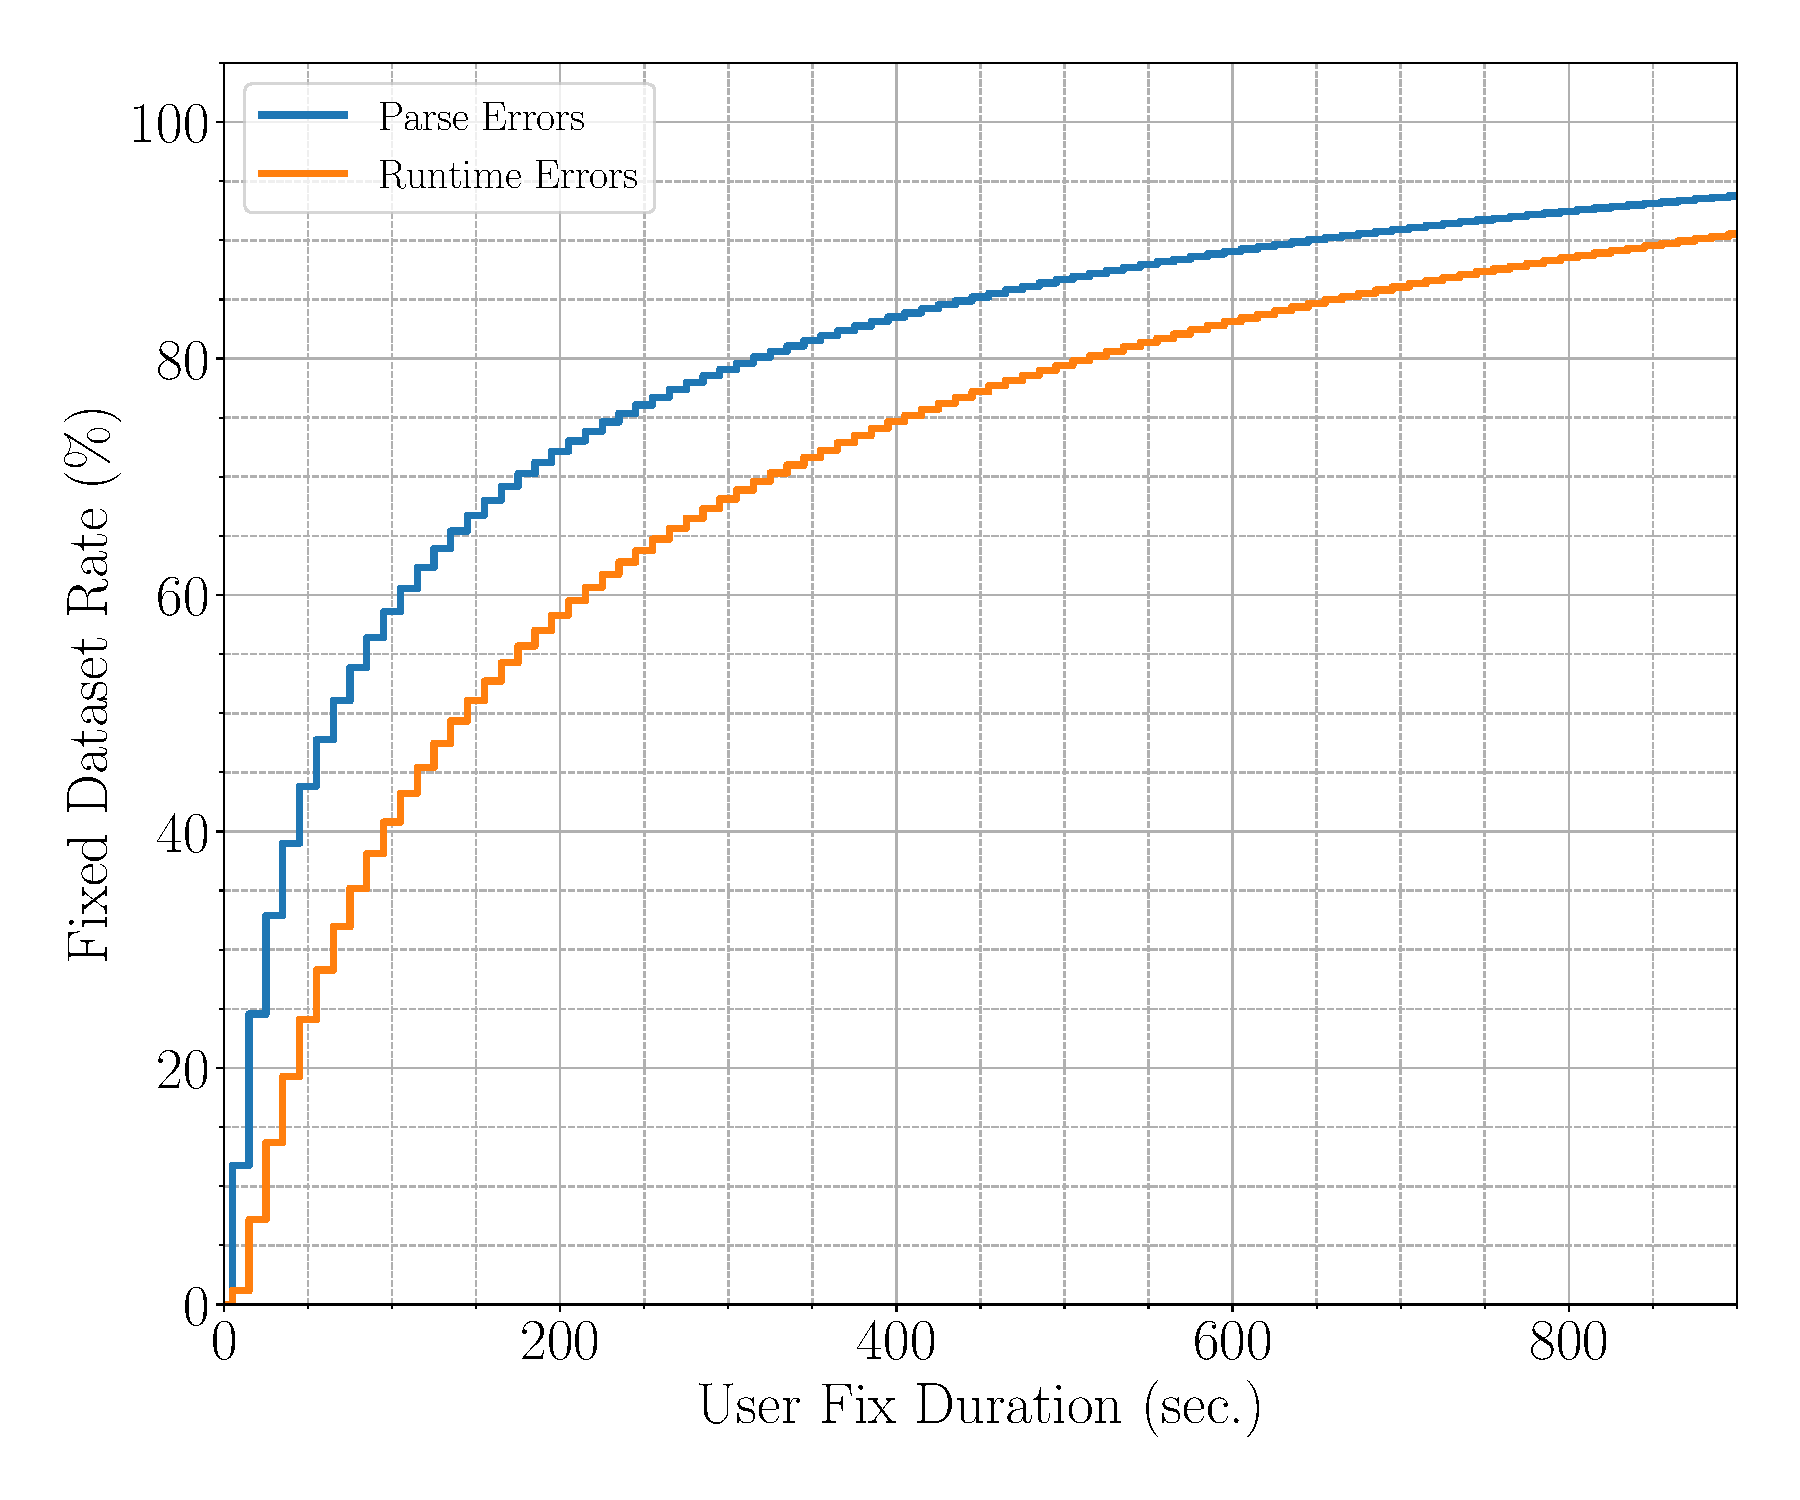
\includegraphics[width=\linewidth]{fixed-rate.pdf}
      \caption{The repair rates of the Python dataset.}
      \label{fig:repair-rate}
  \end{minipage}
\end{figure}

One might imagine that parse (or \emph{syntax}) errors are
usually easier to locate and repair than other algorithmic
or runtime errors \citep{Denny_2012}.
%
For example, the Python parser will immediately inform the programmer
about missing parentheses in function argument lists or for not having
the proper indents in a statement block.
%
However, as has also been shown in previous
work \citep{Ahadi_2018, Kummerfeld2003}, our
data confirms that programmers (especially novices)
deal with these kinds of errors regularly and
spend a considerable amount of time fixing them.

\mypara{Observation 1: Parse errors are very common}
%
\autoref{fig:error-statistics} presents the statistics
of the different types of errors that users encountered
in this dataset.
%
We observe that $77.4 \% $ of all faulty programs failed
with a syntax error, accounting for the vast majority of
the errors that (novice) programmers face with their
programs.
%
The second category is merely $13.6\%$ of the dataset and
represents Python type errors. This is a strong indication
that parse errors are a very common type of error.

\mypara{Observation 2: Parse errors take time to fix}
%
The web-based compiler that we used to generate this
dataset provides us with a \emph{server timestamp}.
%
The timestamp is associated with each program attempt
submission, erroneous or not. The \emph{repair time}
of an erroneous program is calculated by taking the
difference of the two timestamps of the erroneous and
fixed program.
%
This method can be an inaccurate metric of repair time,
as there are various reasons these timings may be exaggerated,
\eg users stepping away from the computer, internet lag \etc.
%
However, in aggregate, due to the large
dataset of program repairs, these timings
can still be viewed as an approximate metric
of the amount of time it took novice programmers to
repair their program errors.

\autoref{fig:repair-rate} shows the \emph{programmer repair rate},
\ie the dataset percentage that is repaired under a given amount of time.
%
It presents the repair rate for parse errors and the rest
of the error types, grouped together here as \emph{runtime} errors.
%
As expected, parse errors are fixed faster than the rest,
but \emph{not by a large difference}.
%
For example, we observe that within 2 minutes,
usually $46\%$ of the runtime errors are repaired, while
around $63\%$ of the syntax errors are.
%
Although, this is a considerable difference,
we observe that there is still a large number
of the ``simpler'' parse errors that required
more than 2 minutes to be fixed.

\begin{figure}[t]
  \centering
  \begin{minipage}[c]{0.48\linewidth}
    \centering
    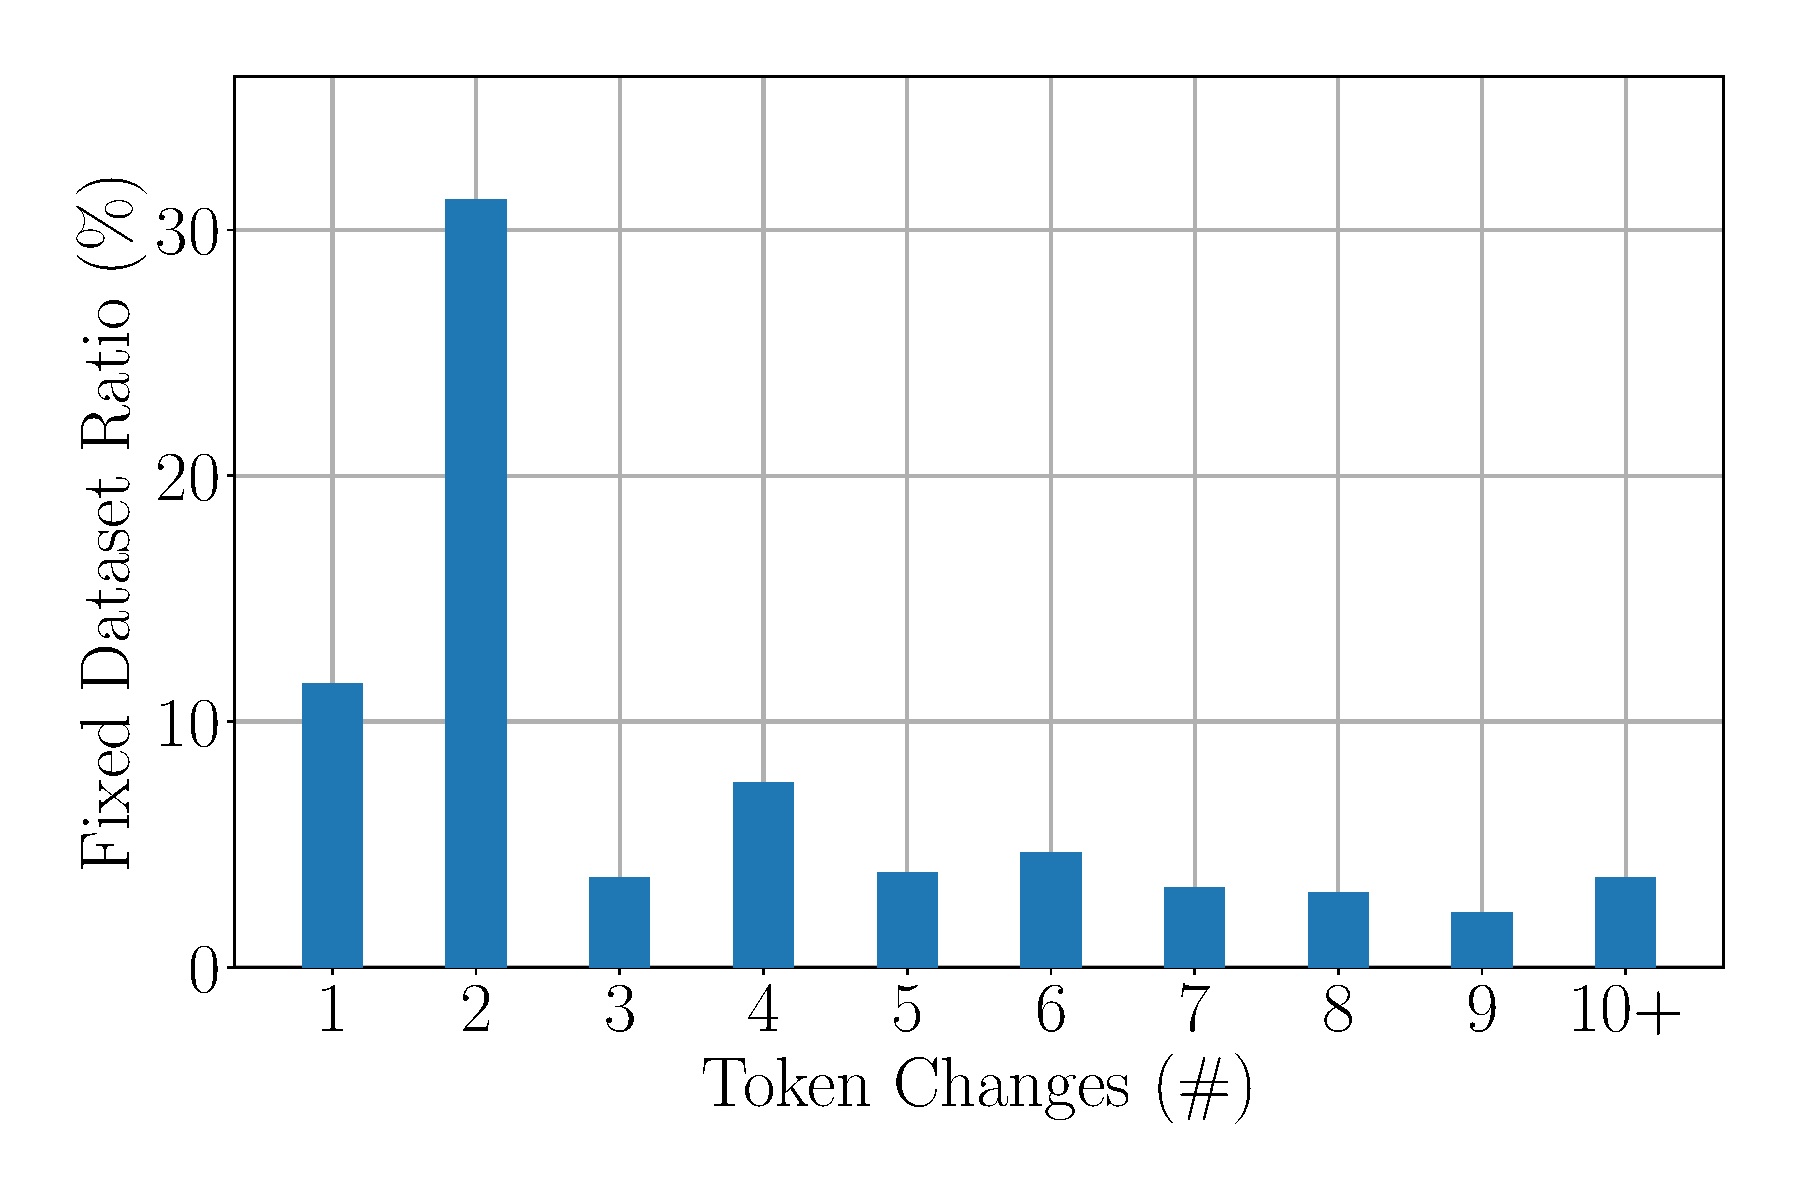
\includegraphics[width=\linewidth]{dataset-ratio-per-change.pdf}
    \caption{The Python dataset ratio that is fixed under the given number of
     token changes.}
    \label{fig:token-changes-ratio}
  \end{minipage}
  \hspace{0.02\linewidth}
  \begin{minipage}[c]{0.48\linewidth}
      \centering
      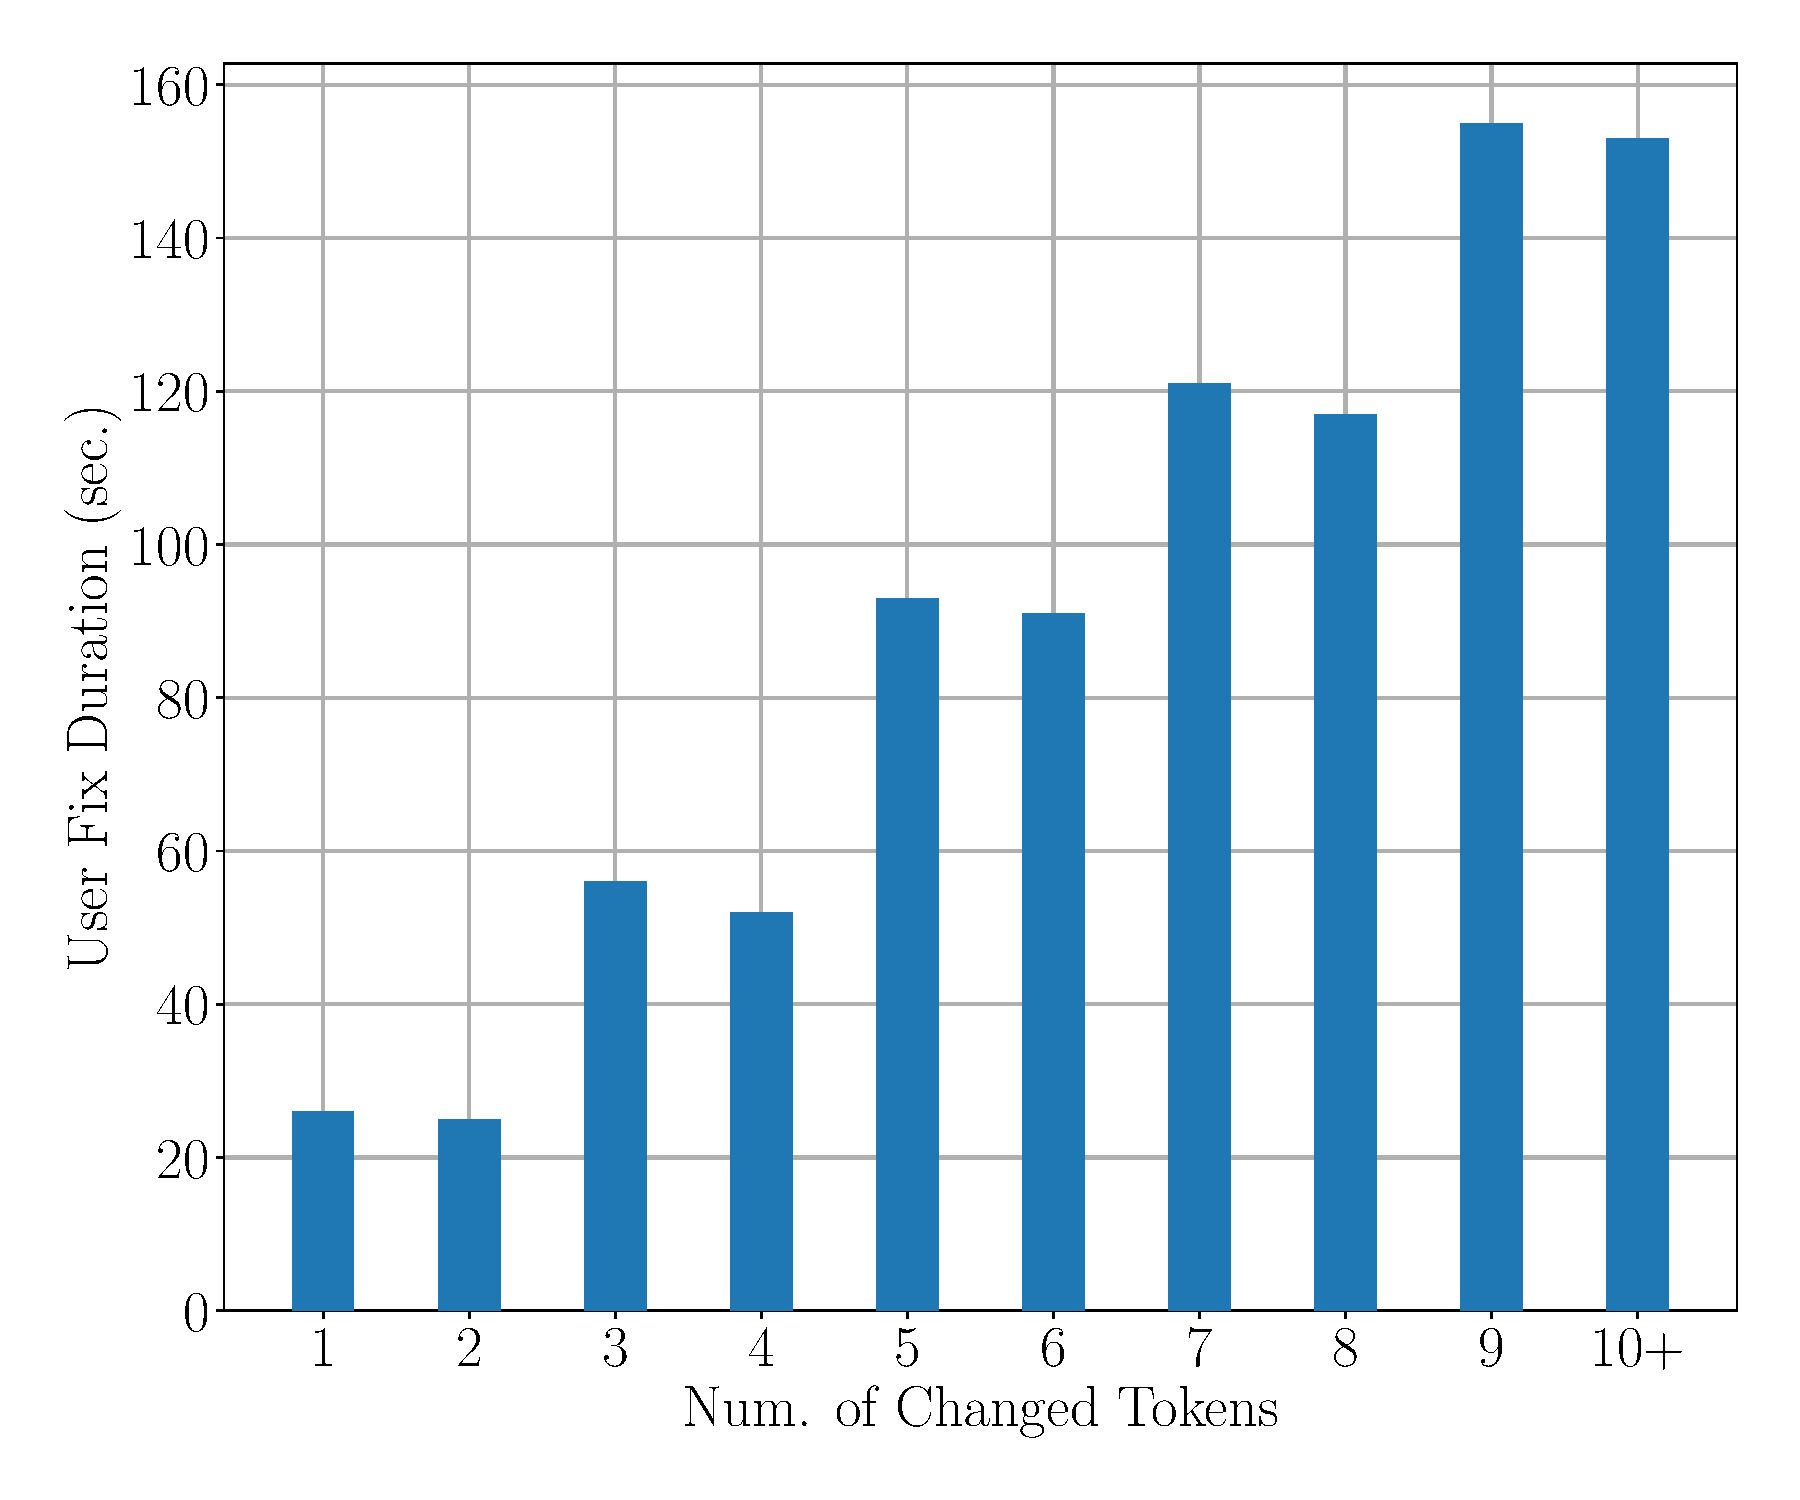
\includegraphics[width=\linewidth]{median-repair-times.pdf}
      \caption{The average time the user needed to fix the erroneous program
      for the needed token changes.}
      \label{fig:token-changes}
  \end{minipage}
\end{figure}

\mypara{Observation 3: Parse errors may need multiple edits to fix}
%
The average \emph{token-level changes} needed to fix a program with syntax
errors, \ie the number of changes in the lexed program token sequence, is
\emph{10.7 token changes}, while the \emph{median is 4}.
%
A variable rename or a different integer are not considered as changes
as they won't affect the syntax error fix.
%
As shown in \autoref{fig:token-changes-ratio}, $14.2\%$ of errors
need only 1 token change, $23.2\%$ need 2 token changes, $7.0\%$
need 3 and $9.0\%$ need 4.
% Ultimately, $53.4\%$ of these errors needs at most 4 token changes to be fixed.
Ultimately, $46.6\%$ of these errors require more than 4 token changes.
%
% It is also important to see how long it takes the users on average to make
% those changes.

\mypara{Observation 4: Parse errors with more edits take longer to fix}
%
\autoref{fig:token-changes} shows the average time that it takes a user to fix
all of their syntax errors per the number of token-level changes in their
programs. As expected, with an increasing number of token changes needed,
programmers need more time to implement those changes. Most importantly, even
for 1 or 2 token changes the average user spends \emph{26 and 25 sec}
respectively, which is still a considerable amount of time for such simple and
short fixes. The repair time jumps to \emph{56 sec} for three token changes.

\smallskip
These four observations indicate that, while some errors can be
easily and quickly fixed by programmers using existing error messages,
there are many cases where novices struggle with fixing syntax errors.
%
Therefore, we can conclude that an automated tool that parses and repairs
such programs in only a few seconds could benefit many novices.

\section{Abstracting Programs with Parse Errors}
\label{sec:prog-abstract}

We start by introducing our approach for abstracting programs with parse errors
into a suitable sequence of tokens for training sequence classifiers. We explain
how a traditional Earley parser can be used to extract partial parses, along
with a Probabilistic Context-Free Grammar (PCFG), in order to get a better level
of abstraction with richer context information than the simple \emph{Lexer}
output.

\begin{figure}[t]
\small
\begin{minipage}[t]{0.42\linewidth}
  \lstDeleteShortInline{|}
  \[
  \boxed{
  \begin{array}{lcl}
    G              & \defeq  & (N,\ \Sigma,\ P,\ S) \\
    \pcfgsym       & \defeq  & (N,\ \Sigma,\ P,\ S,\ W) \\
    \midrule
    G'             & \defeq  & (N',\ \Sigma,\ P',\ S') \\
    P'             & \defeq  & P\ \cup\ \errorrulessym \\
    N'             & \defeq  & N\ \cup\ \{S',\ H,\ I\}\ \cup\\
                   &         & \{E_a\ |\ a \in \Sigma\} \\
    \midrule
    e              & \in    & L(G) \\
    e_{\bot}       & \notin & L(G) \\
    \pairsym       & \defeq & e_{\bot} \times e \\
    \datasetsym    & \defeq & \List{\pairsym} \\
  \end{array}
  }
  \]
  \lstMakeShortInline[language=Python, mathescape=true]{|}
\end{minipage}
\begin{minipage}[t]{0.57\linewidth}
  \lstDeleteShortInline{|}
  \[
  \boxed{
  \begin{array}{lcl}
    \learnPCFGsym  & : & G \to \List{e} \to \pcfgsym \\
    \partialsym    & : & \pcfgsym \to e_{\bot} \to t^a  \\
    \midrule
    \trainDLsym    & : & \List{t^a \times \errorrulessym} \to \Model \\
    \predictDLsym  & : & \Model \to t^a \to \errorrulessym \\
    \midrule
    \diffsym       & : & \pairsym \to \errorrulessym \\
    \ecepsym       & : & \errorrulessym \to e_{\bot} \to e \\
    \trainsym      & : & \datasetsym \to \Model \\
    \predictsym    & : & \Model \to G \to e_{\bot} \to \errorrulessym \\
    \midrule
    \systemsym     & : & G \to \datasetsym \to (e_{\bot} \to e) \\
  \end{array}
  }
  \]
  \lstMakeShortInline[language=Python, mathescape=true]{|}
\end{minipage}
\caption{A high-level API for building a \toolname system that learns parse
error repair function $e_{\bot} \to e$ from a $\datasetsym$ of program pairs.}
\label{fig:api}
\end{figure}


\mypara{Lexical Analysis}
\emph{Lexical analysis}, lexing or tokenization is the process of converting a
sequence of characters \ie a program into a sequence of tokens (strings with an
assigned and thus identified meaning). The program that performs lexical
analysis is called a \emph{lexer} and is usually combined with a parser, which
together analyze the syntax of a programming language $L(G)$, defined by the
grammar $G$. When a program has a syntax error, the output token sequence of the
lexer is the highest level of abstraction that we can acquire for such a
program, since the parser returns with an error, usually with an informative
error message.

\mypara{Token Sequences}
Our goal is to parse a \emph{program token sequence} $t^i$, which is a lexed
program with parse errors (\ie $t^i \notin L(G)$), and repair into a \emph{fixed
token sequence} $t^o \in L(G)$ that can be used to return a repaired program
without syntax errors. Let $t^i$ be a sequence $t^i_1, t^i_2, \dots, t^i_n$ and
$t^o$ be the updated sequence $t^o_1, t^o_2, \dots, t^o_i, \dots, t^o_j, \dots,
t^o_k$. The subsequence $t^o_i, \dots, t^o_j$ is a part of $t^i$ that has been
replaced, deleted or inserted in order to generate the $t^o$. It can be the
whole program, part of it or multiple parts of it. $t^o$ will finally be a token
sequence that can be parsed by the original language's $L(G)$ parser.

However, programs can be large, \ie $n$ can take large values, which makes it
unsuitable for training effectively sequence models. These large programs can
also contain a lot of irrelevant information for fixing a specific parse error.
Therefore, our goal is to first generate an \emph{abstracted token sequence}
$t^a$ that removes all irrelevant information from $t^i$ and gives hints for the
parse error fix by using the internal states of an \emph{Earley} parser.


\subsection{Earley Partial Parses}
\label{sec:prog-abstract:partial}

We propose using an \emph{Earley parser} to generate the abstracted token
sequence $t^a$ for an input program sequence $t^i$. An Earley parser holds
internally a \emph{chart} data structure, \ie \emph{a list of partial parses}.
Given a production rule $X \rightarrow \alpha \beta$, the notation $X
\rightarrow \alpha \cdot \beta$ represents a condition in which $\alpha$ has
already been parsed and $\beta$ is expected and both are sequences of terminal
and non-terminal symbols (tokens).

Each state is a tuple $(X \rightarrow \alpha \cdot \beta,\ j)$, consisting of
\begin{itemize}
    \item the production rule currently being matched $(X \rightarrow \alpha
    \beta)$
    \item the current position in that production (represented by the dot
    $\cdot$)
    \item the origin position $j$ in the input at which the matching of this
    production began
\end{itemize}

We denote the state set at an input position $k$ as $S(k)$. The parser is seeded
with $S(0)$ consisting of only the top-level rule. It then repeatedly executes
three operations: \emph{prediction, scanning,} and \emph{completion}. There
exists a \emph{complete parse} if $(X \rightarrow \gamma \cdot, 0)$ is found in
$S(n)$, where $(X \rightarrow \gamma)$ is the top level-rule and $n$ the input
length. We define a \emph{partial parse} to be any partially completed rules,
\ie if there is $(X \rightarrow \alpha \cdot \beta, i)$ in some state $S(k)$,
where $i < k \leq n$.

Let, again, $t^i_1, t^i_2, \dots, t^i_j, \dots, t^i_k, \dots, t^i_n$ be the
input token sequence $t^i$, where at location $k$ there is a parse error and the
Earley parser has exhausted all possibilities and can not add any more rules in
state $S(k + 1)$. We abstract $t^i$ by getting the longest possible part of the
program that has a partial parse, \ie by finding the largest $j$ for which there
is a rule $(X \rightarrow \alpha \cdot \beta, 0) \in S(j)$. We use this rule for
$X$ to replace $t^i_1, t^i_2, \dots, t^i_j$ in $t^i$ with $\alpha$, thus getting
an abstracted sequence $t^a$. We continue abstracting the program until we reach
the parse error and have no more states available to use, \ie where $S(k + 1) =
\emptyset$. In the same manner, we use the longest possible partial parses that
we can extract from the chart to abstract $t^i_{j+1}, \dots, t^i_k$.

\mypara{Problem: Multiple Partial Parses} Each of the states $S(j)$, where $0
\leq j \leq k$, holds a large number of uncompleted rules, \ie partial parses.
Our heuristic is to choose the longest possible partial parse to abstract our
erroneous programs and thus limit the size of the program token sequence $t^i$
as much as possible. However, it is possible that the longest partial parse
cannot generate abstractions until the position $k$, where $S(k + 1) =
\emptyset$. Additionally, there may be two or more partial parses in $S(k)$,
with different lengths, \eg $\{(X \rightarrow \alpha \cdot \beta,\ j),\ (X'
\rightarrow \alpha' \cdot \beta',\ h)\} \in S(k),\ j \neq h$. In this case, we
want to select the most \emph{probable parse}.

% \mypara{Example} For the running example in \autoref{fig:orig-prog},
% $\{(Arith\_Expr\ \rightarrow\ Literal\ Arith\_Op\ \cdot\ Arith\_Expr,\ 15)$,
% $(Arith\_Expr\ \rightarrow\ Literal\ \cdot,\ 15)\} \in S(17)$, where $S(17)$ is
% the state after the $+$ operator in line 3. Both of those states can lead in
% valid parses, depending how a candidate repair would complete them.


\subsection{Probabilistic Context-Free Grammars}
\label{sec:prog-abstract:pcfg}
We propose learning a \emph{Probabilistic Context-Free Grammar} (PCFG) from a
large corpus of programs $\List{e}, e \in L(G)$, that belong to a language
$L(G)$ that a grammar $G$ defines, as shown in \autoref{fig:api} with
$\learnPCFGsym$. We use the learned PCFG within an augmented Earley parser in
$\partialsym$ to abstract a program $e_{\bot}$ into a abstract token sequence
$t^a$.

\mypara{Learning a PCFG}
A PCFG can be defined similarly to a \emph{context-free grammar} $G \defeq (N,\
\Sigma,\ P,\ S)$ as a quintuple $(N,\ \Sigma,\ P,\ S,\ W)$, where:
\begin{itemize}
    \item $N$ and $\Sigma$ are finite disjoint alphabets of non-terminals and
    terminals, respectively.
    \item $P$ is a finite set of production rules of the form $X \rightarrow
    \alpha$, where $X \in N$ and $\alpha \in (N \cup \Sigma)^{\ast}$.
    \item $S$ is a distinguished start symbol in $N$.
    \item $W$ is a finite set of probabilities $p(X \rightarrow \alpha)$ on
    production rules.
\end{itemize}

Given a dataset of programs $\List{e}, e \in L(G)$ that can be parsed, let
$count(X \rightarrow \alpha)$ be the number of times the production rule $X
\rightarrow \alpha$ has been used to generate a final complete parse, while
parsing $\List{e}$, and $count(X)$ be the number of times the non-terminal $X$
has been seen. The probability for a production rule $X \rightarrow \alpha$ is
then defined as:

\begin{equation*}
    p(X \rightarrow \alpha) = \frac{count(X \rightarrow \alpha)}{count(X)}
\end{equation*}

Of course, under this definition we have the constraint that for any $X \in N$:

\begin{equation*}
    \sum_{X \rightarrow \alpha \in P, \alpha \in (N \cup \Sigma)^{\ast}}{p(X \rightarrow \alpha)} = 1
\end{equation*}

Therefore, $\learnPCFGsym$ invokes an instrumented Earley parser to calculate
all possible counters $count(X \rightarrow \alpha), \forall X \rightarrow
\alpha: P$ and $count(X), \forall X: N$. The instrumented Earley parser keeps a
\emph{global record} for all these counters, while parsing the dataset
$\List{e}$ of programs. Finally, $\learnPCFGsym$ will output a PCFG that is
based on the original grammar $G$ that was used to parse the dataset with the
additional probabilities.

\subsection{From Programs to Abstract Token Sequences}

Given a program $e_{\bot}$ with a parse error and a learned PCFG, $\partialsym$
will generate an abstracted token sequence $t^a$. The PCFG will be used with an
augmented Earley parser to disambiguate partial parses and choose one, in order
to produce an abstracted token sequence as described in
\S~\ref{sec:prog-abstract:partial}.

\mypara{Probabilistic Earley Parsing}
We augment Earley states $(X \rightarrow \alpha \cdot \beta,\ j)$ to $(X
\rightarrow \alpha \cdot \beta,\ j,\ p)$, where $p$ is the probability that $X
\rightarrow \alpha \cdot \beta$ is a correct partial parse. Therefore, the
augmented Earley parser, when we have two (or more) conflicting partial parses
$\{(X \rightarrow \alpha \cdot \beta,\ j,\ p),\ (X' \rightarrow \alpha' \cdot
\beta',\ h,\ p')\} \in S(k)$, selects the partial parse with the highest
probability $max(p,\ p')$. The augmented Earley parser calculates the
probability $p$ for a partial parse $(X \rightarrow \alpha \cdot \beta,\ j,\ p)$
in the state $S(k)$, as the product $p_1 \cdot p_2 \cdot \dots \cdot p_{k-1}$ of
the probabilities $p_1,\ p_2,\ \dots,\ p_{k-1}$ that are associated with the
production rules $(X_1 \rightarrow \alpha_1 \cdot \beta_1,\ i_1,\ p_1), (X_2
\rightarrow \alpha_2 \cdot \beta_2,\ i_2,\ p_2), \dots$ that have been used so
far to parse the string of tokens $\alpha$.

% \mypara{Example: Selecting Most Likely Partial Parse}




\section{Training Sequence Classifiers}
\label{sec:seq-classifiers}

Our next task is to \emph{train} a model that can predict the error production
rules that are needed to parse a given program $e_{\bot}$ (with syntax errors)
according to a given grammar $G$, by using its (abstracted) program token
sequence $t^a$.
%
We define the function $\predictDLsym$ which takes as input a \emph{pre-trained
sequence classifier} $\Model$ and an abstracted token sequence $t^a$ and returns
as output a \emph{small subset} of $\errorrulessym$.
%
We train the $\Model$ offline with the $\trainDLsym$ method with a dataset
$\List{t^a \times \errorrulessym}$ of token sequences $t^a$ and the \emph{exact
small set} of error production rules $\errorrulessym$ that the ECE-Parser used
to generate the \emph{user parse}. We build our classifier $\Model$ using
classic \emph{Deep Neural Networks (\dnn{}s)} and parts of state-of-the-art
\emph{Sequence-to-Sequence (seq2seq)} models. We leave the high level details of
acquiring the dataset of labeled token sequences and using the predictor for new
erroneous programs for \autoref{sec:whole-system}. In the next few paragraphs,
we summarize the recent advances in machine learning that help as build the
sequence classifier.

We encode the task of learning a function that will map token sequences of
erroneous programs to a small set of error production rules as a
\emph{supervised multi-class classification (MCC)} problem. A \emph{supervised}
learning problem is one where, given a labeled training set, the task is to
learn a function that accurately maps the inputs to output labels and
generalizes to future inputs. In a \emph{classification} problem, the function
we are trying to learn maps inputs to a discrete set of two or more output
labels, called \emph{classes}. We use an \emph{Transformer encoder} to encode
the input sequences into abstract vectors that we then directly feed into a
\emph{\dnn} classifier to build a \emph{Transformer classifier}.

\mypara{Neural Networks}
A neural network can be represented as a directed acyclic graph whose nodes are
arranged in layers that are fully connected by weighted edges. The first layer
corresponds to the input features, and the final to the output. The output of an
internal node is the sum of the weighted outputs of the previous layer passed to
a non-linear \emph{activation function}, which in recent work is commonly chosen
to be the rectified linear unit (ReLU) \citep{Nair2010-xg}. In this work, we use
relatively \emph{deep neural networks} (\dnn) that have proven to make more
accurate predictions in recent work~\citep{Schmidhuber_2015}. A thorough
introduction to neural networks is beyond the scope of this
work~\citep{Hastie2009-bn, Nielsen2015-pu}.

% For example, the outputs of an internal layer of nodes $l$ is given as $y_l =
% g(W_{l-1} y_{l-1})$, where $W_{l-1}$ is the weight matrix for the edges between
% layers $l$ and $l-1$ and $y_{l-1}$ is the output of the previous layer. The
% input $y_0 = x$ is the input features of the neural network and, finally, g is
% the activation function, which in recent work is commonly chosen to be the
% rectified linear unit (ReLU), defined as $g(x) = max(0, x)$ \citep{Nair2010-xg}.
% The number of layers, the number of nodes per layer, and the connections between
% layers constitute the \emph{architecture} of a neural network

\mypara{Sequence Models}
\emph{Seq2seq} models aim to transform input sequences of one domain into
sequences of another domain \citep{Sutskever_2014}. In the general case, these
models consist of two major layers, an \emph{encoder} and a \emph{decoder}. The
encoder transforms an input token sequence $x_1, x_2, \dots, x_n$ into a
\emph{abstract vector} $V \in \R^k$ that captures all the essence and context of
the input sequence. This vector doesn't necessarily have some physical meaning
and is just an internal representation of the input sequence into a higher
dimensional space. The abstract vector is then given as an input to the decoder,
which in turn transforms it into an output sequence $y_1, y_2, \dots, y_n$.

% \begin{align}
%     h_t &= f(W_{hx} x_t + W_{hh} h_{t-1}) \label{eq:1} \\
%     y_t &= g(W_{yh} h_t) \label{eq:2}
% \end{align}

The simplest approach historically uses a Recurrent Neural Network (RNN)
\citep{Rumelhart1986, Werbos1990}, which is a natural next step from the classic
neural networks. Each RNN unit operates on each input token $x_t$ separately. It
keeps an internal \emph{hidden state} $h_t$ that is calculated as
% in $h_t = f(W_{hx} x_t + W_{hh} h_{t-1})$,
a function of the input token $x_t$ and the previous hidden state $h_{t-1}$.
% The weight matrices $W_{hx}$ and $W_{hh}$ parametrize the input-to-hidden and
% the hidden-to-hidden connections respectively. The function $f$ is another
% non-linear activation function such as \emph{tanh, sigmoid} and \emph{ReLU}.
The output $y_t$ is calculated as
% $y_t = g(W_{yh} h_t)$, \ie
the product of the current hidden state $h_t$ and an output weight matrix. The
activation function is usually chosen as the standard \emph{softmax} function
\citep{Goodfellow-et-al-2016, Bishop-book-2006}. Softmax assigns probabilities
to each output that must add up to 1.
% which, for an output vector $y = (y_1, \dots, y_N) \in \R^{N}$, is defined as:
% \[ \sigma(y)_i = \frac{e^{y_i}}{\sum_{j=1}^{N} e^{y_j}},\ for\ i = 1, \dots, N.
% \]
Finally, the loss function at all steps of the RNN is typically calculated as
the sum of the cross-entropy loss of each step.

% These recurrent models have to generate the sequence of hidden states $h_t$, as
% a function of the previous hidden state $h_{t-1}$ and the input $x_t$. This
% sequential generation of hidden states limits parallelization within training
% examples and causes training problems when dealing with longer sequences, as
% memory constraints limit batching across examples. However, the latest
% state-of-the-art approach for seq2seq architectures is the newer
% \emph{Transformer} model \citep{Vaswani_2017} that replaces the classic RNN unit
% and solves these problems due to its \emph{attention mechanisms}.

\mypara{Transformers}
The Transformer is an \dnn architecture that deviates from the recurrent pattern
(\eg RNNs) and is solely relying on \emph{attention mechanisms}. Attention has
been of interest lately \citep{Bahdanau2015, Kim2017, Vaswani_2017} mainly due
to its ability to detect dependencies in the input or output sequences
regardless the distance of the tokens. The nature of this architecture makes the
Transformer significantly more easy to parallelize and has as a result a higher
quality of predictions and sequence translations after only being trained for a
small amount of time.

The novel architecture of a Transformer \citep{Vaswani_2017} is structured as a
\emph{stack of $N$ identical layers}. Each layer has two main sub-layers. The
first is a \emph{multi-head self-attention mechanism}, and the second is a
position-wise fully connected neural network. The output of each sub-layer is
$LayerNorm(x + SubLayer(x))$, where $SubLayer(x)$ is the function implemented by
each sub-layer, followed by a residual connection around each of the two
sub-layers and  by layer normalization $LayerNorm(x)$. To facilitate these
residual connections, all sub-layers in the model, as well as the input
\emph{embedding layers}, produce outputs of the same dimension $d_{model}$.

% This architecture is used as described above in a seq2seq model
% \citep{Vaswani_2017} for the encoder. The decoder would require an extra third
% sub-layer, which performs multi-head attention over the output of the encoder
% stack. However, in our task we learn sets of error production rules, which we
% frame as a classic \emph{multi-class classification} problem. We are dealing
% with input sequences of varied sizes, where no straightforward feature
% extraction technique exists. Therefore, we utilize the effectiveness of the
% state-of-the-art \emph{Transformer encoder} to summarize the programs into
% fixed-length vectors that can then be fed into classic \dnn{} classifiers.

% \subsection{Transformer Classifier}
% \label{sec:seq-classifiers:location-rank}


% \mypara{Multi-class \dnn{}s}
%
% A \dnn can be used as a binary classifier, \ie predict if the given input
% belongs into a class or not. While this model is enough for many tasks, \eg
% error localization \citep{Sakkas_2020, Seidel:2017}, in the case of error rule
% prediction we have to select from multiple \emph{classes}. We therefore use a
% \dnn for our error rule prediction $\Model$, but we adjust the output layer to
% have $N$ nodes for the selected $N$ error-rule-classes.

% \mypara{Multi-class Transformer Classifiers}
%
\mypara{Transformer Classifier}
For our task, we choose to structure $\Model$ as a \emph{Transformer
Classifier}. We use a novel Transformer encoder to represent an abstracted token
sequence $t^a = (t^a_1, t^a_2, \dots, t^a_n)$ into an abstract vector $V \in
\R^k$. The abstract vector $V$ is then fed as input into a multi-class \dnn. We
use $\trainDLsym$ to train the $\Model$ given the training set $\List{t^a \times
\errorrulessym}$. The binary cross-entropy loss function is used per class to
assign the loss per training cycle. $\Model$ is used to predict error production
rules for a new input program $t^a$. Critically, we require that the classifier
outputs a \emph{confidence score} $\Conf$ for each possible error rule that
measures how sure the classifier is that the rule can be used to parse the
associated input program $e_{\bot}$. The $\predictDLsym$ function uses the
trained $\Model$ to predict the confidence scores $\List{\errorrulessym\ \times\
\Conf}$ for every error production rule $\errorrulessym$ for a new unknown
program $e_\bot$ with syntax errors. The $\errorrulessym$ are then sorted based
on their predicted confidence score $\Conf$ and finally the \emph{top-N} rules
are returned for error-correcting parsing. $N$ is a small number in the 10s that
will give accurate predictions without making the ECE-Parser too slow, as we
discuss in \autoref{sec:eval}.

\section{Building a fast error-correcting parser}
\label{sec:whole-system}

We show how $\systemsym$ uses the abstracted token sequences from
\autoref{sec:prog-abstract} and the trained sequence models from
\autoref{sec:seq-classifiers} to generate an \emph{error-correcting parser}
$(e_{\bot} \to e)$, that takes as input a program $e_{\bot}$ with parse errors,
parsers it, and produces a correct program $e$.


\subsection{Learning Error Production Rules}
\label{sec:whole-system:error-rules}

\mypara{Extracting error rules efficiently from a dataset}


\subsection{Training the Classifier}
\label{sec:whole-system:training-classifier}

\mypara{Training the Transformer Classifier}

\mypara{Predicting Error Rules}

\subsection{Generating an error-correcting parser}
\label{sec:whole-system:building-ecp}

\section{Evaluation}
\label{sec:eval}

We have implemented our approach in \toolname: a system for repairing parse
errors for \python at its entirety. Next, we describe our implementation and an
evaluation that addresses four questions:

\begin{itemize}
    \item \textbf{RQ1}: How \emph{accurate} are \toolname's predicted error production rules?
                        (\S~\ref{sec:eval:accuracy})
    \item \textbf{RQ2}: How \emph{precisely} can \toolname repair parse errors?
                        (\S~\ref{sec:eval:precise})
    \item \textbf{RQ3}: How \emph{efficiently} can \toolname repair parse errors?
                        (\S~\ref{sec:eval:efficiency})
    \item \textbf{RQ4}: How \emph{useful} are \toolname's suggested repairs?
                        (\S~\ref{sec:eval:useful})
\end{itemize}

% \subsection{Implementation} \label{sec:eval:gen_method}

\mypara{Training Dataset}
For our evaluation, we use the \python dataset we used in our error data
analysis in \autoref{sec:error-analysis} gathered from
PythonTutor.com~\citep{Guo2013} between the years 2017 and 2018. The dataset has
more than 1,100,000 usable erroneous Python programs and their respective fixes.
The programs have an average length of \emph{87 tokens}, while the abstracted
token sequences have a much shorter average of \emph{43 tokens}. We choose
15,000 random programs from the dataset for all our tests, and the rest we use
as our training set.

We first learn a PCFG on the training set of fixed programs in order to learn
the probabilities for each production rule in the \emph{full set of the \python
grammar}. \toolname then extracts the abstracted token sequences for all
programs in the training set. Next, while for the full set of \python there are
\emph{455 possible terminal error production rules} that \toolname's can predict
from, in reality only \emph{340 error rules} are ever used in the full dataset.
We arrive at this set of error rules by parsing all the erroneous programs in
the training set with the ECE-Parser and the "diff" error rules, as described in
\autoref{sec:overview:train}. Each program is also assigned as labels these
error rules that make the ECE-Parser parse the erroneous program successfully.

\mypara{Transformer Classifier}
\toolname's error rule prediction uses a Transformer classifier with \emph{six}
transformer blocks, that each has a fully-connected hidden layer of 256 neurons
and 12 attention heads. The output of the transformer blocks is then connected
to a \dnn based classifier with \emph{two} fully-connected hidden layers of 256
and 128 neurons respectively. The neurons use rectified linear units (ReLU) as
their activation function \citep{Nair2010-xg}, while the output layer uses the
sigmoid function for each class \citep{Nielsen2015-pu}. Additionally, the are
\emph{two input embedding layers} of a length of 128, one for input tokens and
one for their positions in the sequence. We also limit the size of the input
abstracted token sequences to a length of 128, which covers $95.7\%$ of the
training set, without the need of pruning them. Finally, the Transformer
classifier was trained using an \textsc{Adam} optimizer \citep{Kingma2014-ng}, a
variant of stochastic gradient descent that converges faster, for a total of 50
epochs.

\subsection{RQ1: Accuracy}
\label{sec:eval:accuracy}

% colors from http://colorbrewer2.org/?type=sequential&scheme=Blues&n=3
\definecolor{blue1}{HTML}{DEEBF7}
\definecolor{blue2}{HTML}{9ECAE1}
\definecolor{blue3}{HTML}{3182BD}
\definecolor{green1}{HTML}{E5F5E0}
\definecolor{green2}{HTML}{A1D99B}
\definecolor{green3}{HTML}{31A354}

\begin{figure}[t]
  % \begin{minipage}[c]{0.49\linewidth}
    \centering
    \resizebox{0.6\linewidth}{!}{
      \Large
      \begin{tikzpicture}
      \begin{axis}[
        ybar stacked,
        width=1.1\linewidth,
        height=11cm,
        % title={Accuracy of Repair Template Prediction},
        ylabel={Prediction Accuracy (\%)},
        bar width=1cm,
        ymin=0.0,
        ymax=101.0,
        ytick={0.0, 10.0, 20.0, 30.0, 40.0, 50.0, 60.0, 70.0, 80.0, 90.0, 100.0},
        yticklabel={\pgfmathparse{\tick}\pgfmathprintnumber{\pgfmathresult}},
        ytick style={draw=none},
        ymajorgrids = true,
        symbolic x coords={original, abstracted, abstracted-best},
        enlarge x limits=0.3,
        xtick=data,
        xtick style={draw=none},
        xticklabels={\textsc{Original}\xspace, \textsc{Abstracted}\xspace, \textsc{Threshold}\xspace},
        %x tick label style={rotate=45, anchor=north east},
        % x tick label style={font=\small},
        % y tick label style={font=\small},
        reverse legend,
        % transpose legend,
        legend style={legend pos = north east, legend columns=4, font=\small},
      ]

      \addplot[draw=black, fill=blue2, bar shift=-.501cm, postaction= { pattern=dots }] coordinates {(original, 0.0) (abstracted, 0.0) (abstracted-best, 79.28025102961365)};

      \resetstackedplots

      \addplot[draw=black, fill=green2, bar shift=.501cm, postaction= { pattern=dots }] coordinates {(original, 0.0) (abstracted, 0.0) (abstracted-best, 69.82968369829683)};

      \resetstackedplots

      \addplot[draw=black, fill=green1, bar shift=.501cm] coordinates {(original, 12.875536480686696) (abstracted, 58.394160583941606) (abstracted-best, 0.0)};
      \addlegendentry{Top-10}
      \addplot[draw=black, fill=green2, bar shift=.501cm] coordinates {(original, 20.100143061516448) (abstracted, 14.922952149229523) (abstracted-best, 0.0)};
      \addlegendentry{Top-20}
      \addplot[draw=black, fill=green3, bar shift=.501cm] coordinates {(original, 31.974248927038623) (abstracted, 15.49067315490673) (abstracted-best, 0.0)};
      \addlegendentry{Top-50}
      \addlegendimage{empty legend}
      \addlegendentry{Rare:}

      \resetstackedplots

      \addplot[draw=black, fill=blue1, bar shift=-.501cm] coordinates {(original, 56.712132089016514) (abstracted, 72.11217885859972) (abstracted-best, 0.0)};
      \addlegendentry{Top-10}
      \addplot[draw=black, fill=blue2, bar shift=-.501cm] coordinates {(original, 11.769733018835673) (abstracted, 9.335163757599531) (abstracted-best, 0.0)};
      \addlegendentry{Top-20}
      \addplot[draw=black, fill=blue3, bar shift=-.501cm] coordinates {(original, 18.65107852186101) (abstracted, 11.253840622344256) (abstracted-best, 0.0)};
      \addlegendentry{Top-50}
      \addlegendimage{empty legend}
      \addlegendentry{All:}

      \end{axis}
      \end{tikzpicture}
    }
    \caption{
      Results of our error production rule prediction classifiers for the simple original token sequences and their abstracted versions using the PCFG.
    }
    \label{fig:accuracy-results}
  % \end{minipage}
  % \begin{minipage}[c]{0.49\linewidth}
  %   \centering
  %   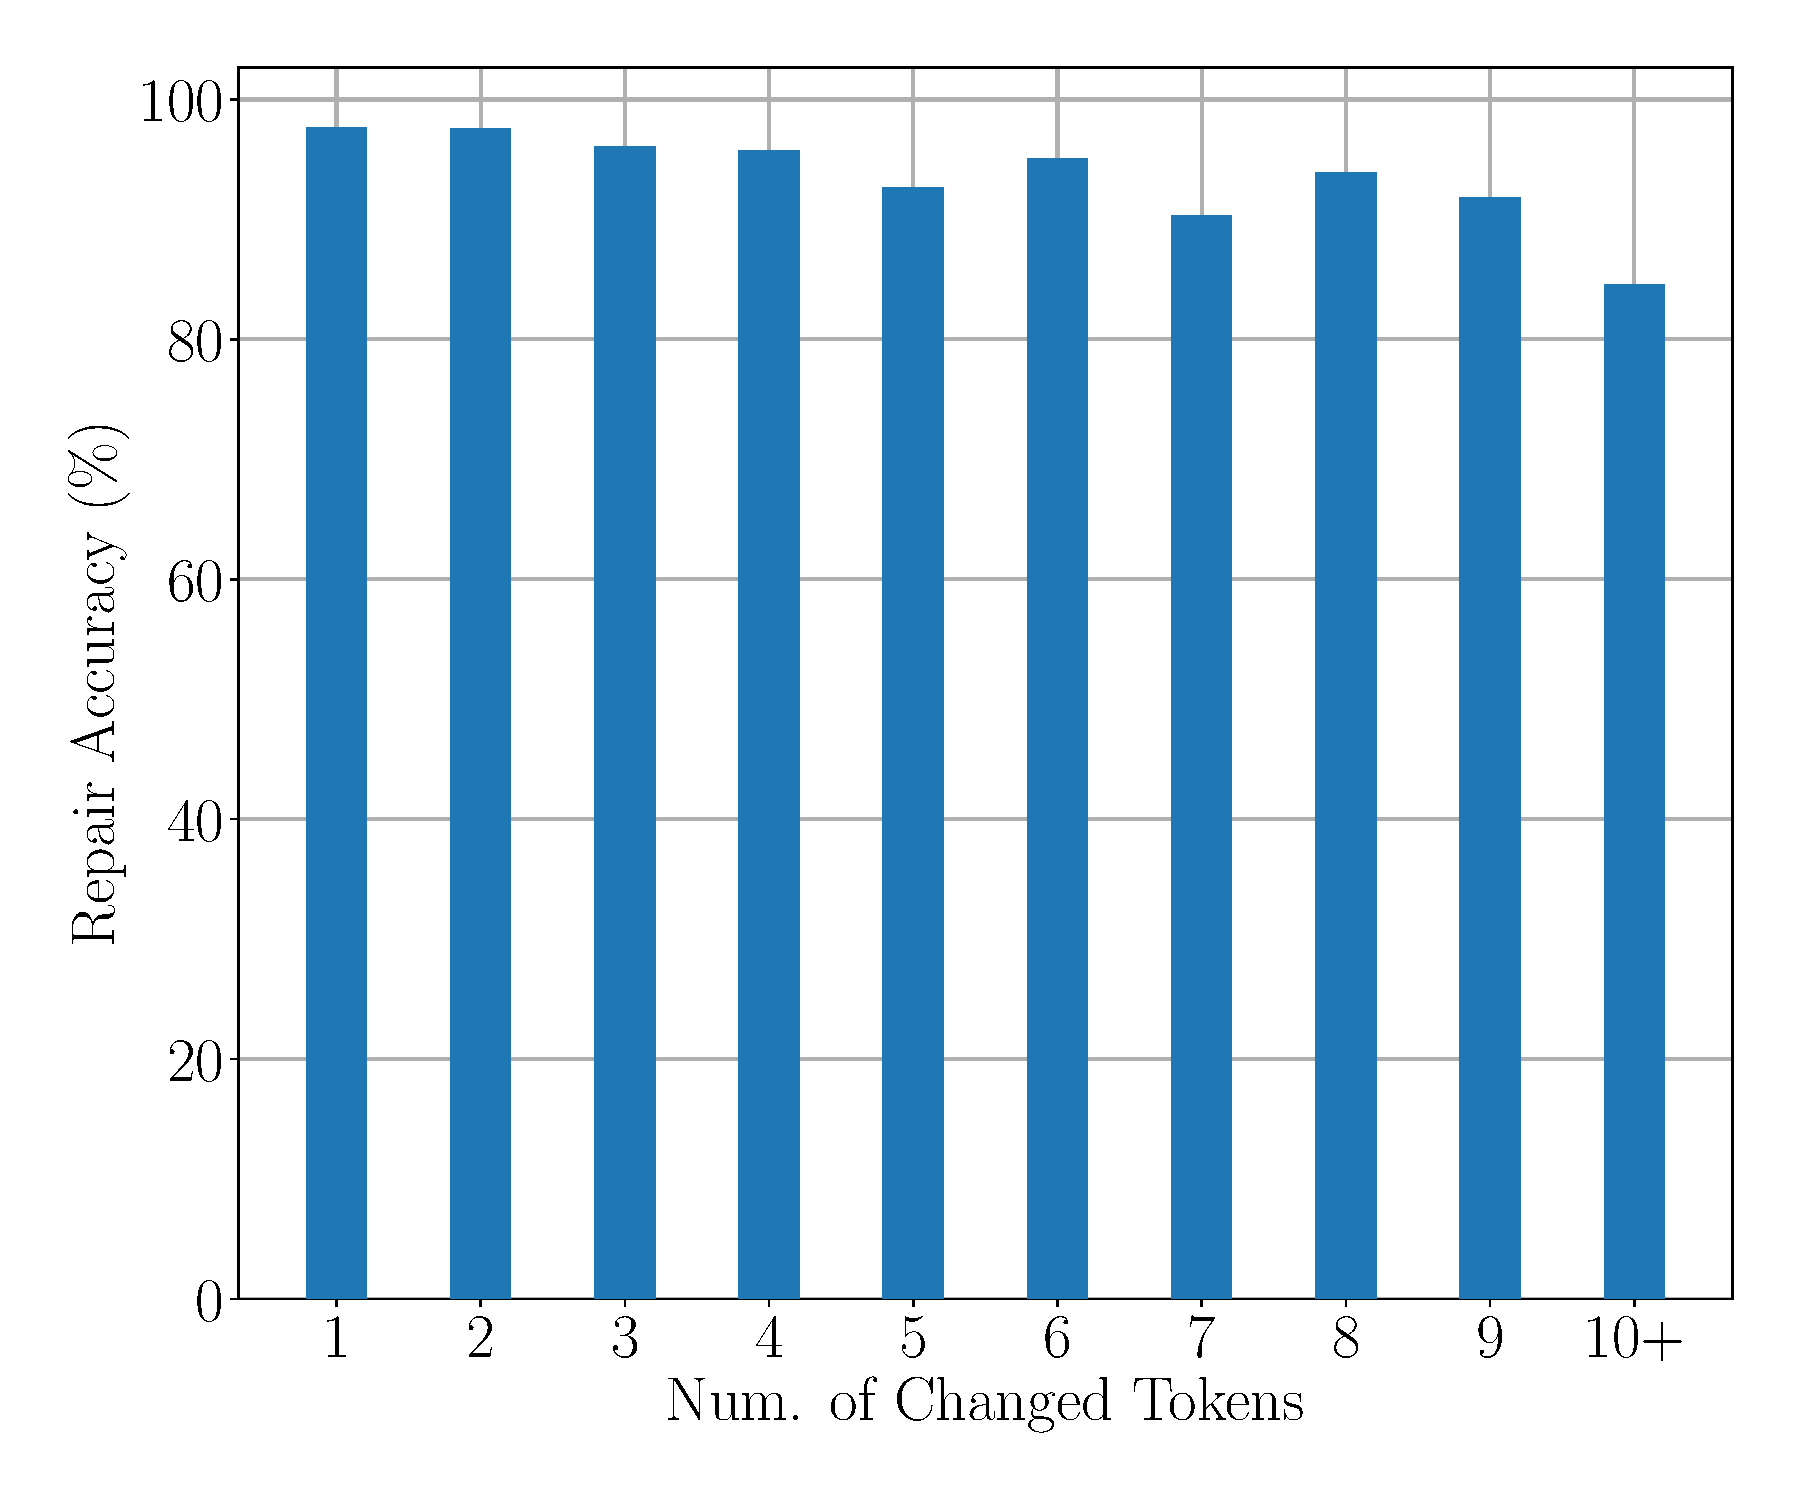
\includegraphics[width=\linewidth]{accuracy-per-change.pdf}
  %   \caption{The repair accuracy for the number of edits needed by the user to repair.}
  %   \label{fig:accuracies-per-changes}
  % \end{minipage}
\end{figure}


% \mypara{Results: Accuracy of Error Rule Prediction}
%
\autoref{fig:accuracy-results} shows the accuracy results of our error
production rule prediction experiments. The y-axis describes the
\emph{prediction accuracy}, \ie the fraction of test programs for which the
correct \emph{full set} of error rules to repair the program was predicted in
the top-K sorted rules.
%
The \textsc{Original} version of our transformer classifier does not consider
the abstracted token sequences and used the full \textsc{Original} token
sequences, whose results are presented in the first two bars of
\autoref{fig:accuracy-results}. The next two bars show our final results using
the \textsc{Abstracted} token sequences to train the classifier. Finally, the
last two dotted bars show the results for when a \textsc{Threshold} is set in
order to select the predicted error rules, instead of picking the static top-K
ones. The predicted error rule set can have a size anywhere between 1 and a
maximum of 25 (pre-defined by us based on the top-K results).

The blue bars show the accuracy on the full test set of \textsc{All} 15,000 test
programs, while the green bars show the results on the subset of the
\textsc{Rare} programs, \ie the programs that did not include any of the 50 most
popular error rules, that amount only for 4.8\% of our test set.

The \textsc{Original} predictor, even with the Top-50 predicted error rules is
less accurate than the Top-20 predictions of the \textsc{Abstracted}, with an
accuracy of 87.13\%, which drops to 68.48\% and 56.71\% respectively for the
Top-20 and Top-10 predictions. The \textsc{Abstracted} predictor significantly
outperforms the \textsc{Original} predictor with a 72.11\% Top-10 accuracy,
81.45\% Top-20 accuracy and 92.70\% Top-50 accuracy.

The \textsc{Threshold} predictions are almost as accurate as the
\textsc{Abstracted} Top-20 predictions with an accuracy of 79.14\% and a median
number of selected error rules of 11 (average 13.2). This could potentially mean
that this predictor is a valid alternative for the static Top-20 predictions.

Finally, we observe that our \textsc{Abstracted} classifiers generalize
efficiently for our dataset of erroneous \python programs and is almost as
accurate for the \textsc{Rare} programs as the rest of the dataset with a
73.32\% Top-20 accuracy (88.81\% Top-50 accuracy). The same holds for the
\textsc{Threshold} predictions with a 66.42\% accuracy.

\begin{framed}
  \noindent \toolname's transformer classifier learns to encode programs with
  syntax errors and select candidate error production rules for them
  effectively, yielding \emph{high accuracies}. By abstracting the tokens
  sequences, \toolname is able to \emph{generalize} better and make more
  accurate predictions with a \emph{81.45\% Top-20 accuracy}.
\end{framed}


\subsection{RQ2: Repaired Program Preciseness}
\label{sec:eval:precise}

Next we evaluate \toolname's end-to-end accuracy and preciseness in generating
valid parses for programs with syntax errors. For all of our tests we limit
\toolname's parsing time to \emph{5 mins} and run our experiments on the 15,000
program  test set. Additionally, we use here the highest-performing transformer
classifier, the \textsc{Abstracted} classifier.

We compare \emph{two versions} of our implementation of \toolname
(\textsc{AllParses} and \textsc{MinimumCost}) against two versions of the
error-correcting parser with a static selection of the 20 and 50 most popular
error production rules in our training set. We make this comparison because we
observe in our training set that the 50 most of popular error rules are used for
parsing as much as \emph{86\%} of the dataset.

Our \textsc{AllParses} ECE-Parser and \textsc{MinimumCost} ECE-Parser both use
the \emph{Top-20 predictions} from our \textsc{Abstracted} classifier to parse
and repair buggy programs. The \textsc{AllParses} ECE-Parser keeps internally
\emph{all possible states} that arise from using the predicted error rules
similarly to the original ECE-Parser described in \citep{Aho_1972}. We use a
maximum repair cost of 2 edits (\ie a maximum of 2 insertions, deletions or
replacements) to limit the search space. The \textsc{MinimumCost} version
however keeps always the minimum-edit repair and discards all other states that
may lead to a higher cost. This allows for a higher maximum cost of 10 edits.
Finally, while \textsc{AllParses} can generate a large number of repairs, we
keep only the top 3 repairs after filtering with a static code checker
(\textsc{Pylint}, \url{https://www.pylint.org/}) as most developers will
consider at most five suggestions before falling back to manual debugging
\citep{Kochhar2016-oc, Parnin2011-ce}.

\autoref{tab:seq2parse_full_results} shows the percentage of test programs that
each of these four versions can parse successfully (\ie the parse accuracy), the
rare programs parse accuracy and the amount of parses that match the one that
user compiled. We observe that the Top-20 predictions with the
\textsc{MinimumCost} ECE-Parser \emph{outperforms} every other option with
94.25\% parse accuracy and 94.01\% rare parse accuracy. It also achieves to
generate the intended user parse for 20.55\% of the set, \ie over 1 out 5 of the
cases. The 20 most popular ECE-Parser with 79.87\% parse accuracy and 65.01\%
rare parse accuracy is much less accurate, and achieves 4.24\% less times to
generate the user parse, while the 50 most popular is slightly less accurate
with 91.91\% and 82.70\% accuracy, as expected from the usage of a large number
of popular error rules. The 50 most popular ECE-Parser has also a high user fix
accuracy of 18.61\%. The \textsc{AllParses} ECE-Parser has a lower parse
accuracy of 61.82\% in general, however it manages to generate the user fix
33.92\% of the times and achieve a 72.22\% rare accuracy. It thus achieves to
parse one out of three programs with syntax errors, while also being effective
to parse even the rare programs.

\begin{framed}
  \noindent \toolname can \emph{parse and repair 94.25\%} of programs with
  syntax errors, while also generating \emph{the user fix over 1 out 5 of
  cases}.
\end{framed}

% \begin{table}[t]
%   \centering
%   \begin{tabular}{l||cccc}
%     Error Rule Approach            & Parse Accuracy & User Parse Rate & Parse time & Speedup \\
%     \hline
%     20 Most Popular                & 79.81\% & 16.31\% & 4.8 sec  & 45.8 sec \\
%     50 Most Popular                & 90.03\% & 18.55\% & 10.6 sec & 37.1 sec \\
%     Top-20 (\textsc{AllParses})   & 59.31\% & 30.57\% & 15.6 sec & 57.4 sec \\
%     Top-20 (\textsc{MinimumCost}) & 92.45\% & 19.95\% & 5.3 sec  & 68.0 sec \\
%   \end{tabular}
%   \caption{Experimental results of \toolname's repair approaches.}
%   \label{tab:seq2parse_full_results}
% \end{table}

\begin{figure}[t]
  \centering
  \begin{minipage}[c]{0.46\linewidth}
    \centering
    \resizebox{\linewidth}{!}{
      \begin{tabular}{l||ccc}
        Error Rule            & Parse            & Rare Parse       & User Fix \\
        Approach              & Accuracy         & Accuracy         & Accuracy \\
        \hline
        20 Most Popular       & 79.87\%          & 65.01\%          & 16.31\% \\
        50 Most Popular       & 91.91\%          & 82.70\%          & 18.61\% \\
        \textsc{AllParses}    & 61.82\%          & 72.22\%          & \textbf{33.92\%} \\
        \textsc{MinimumCost}  & \textbf{94.25\%} & \textbf{94.01\%} & 20.55\% \\
      \end{tabular}
    }
    \caption{Experimental results of \toolname's repair approaches.}
    \label{tab:seq2parse_full_results}
  \end{minipage}
  \begin{minipage}[c]{0.53\linewidth}
    \centering
    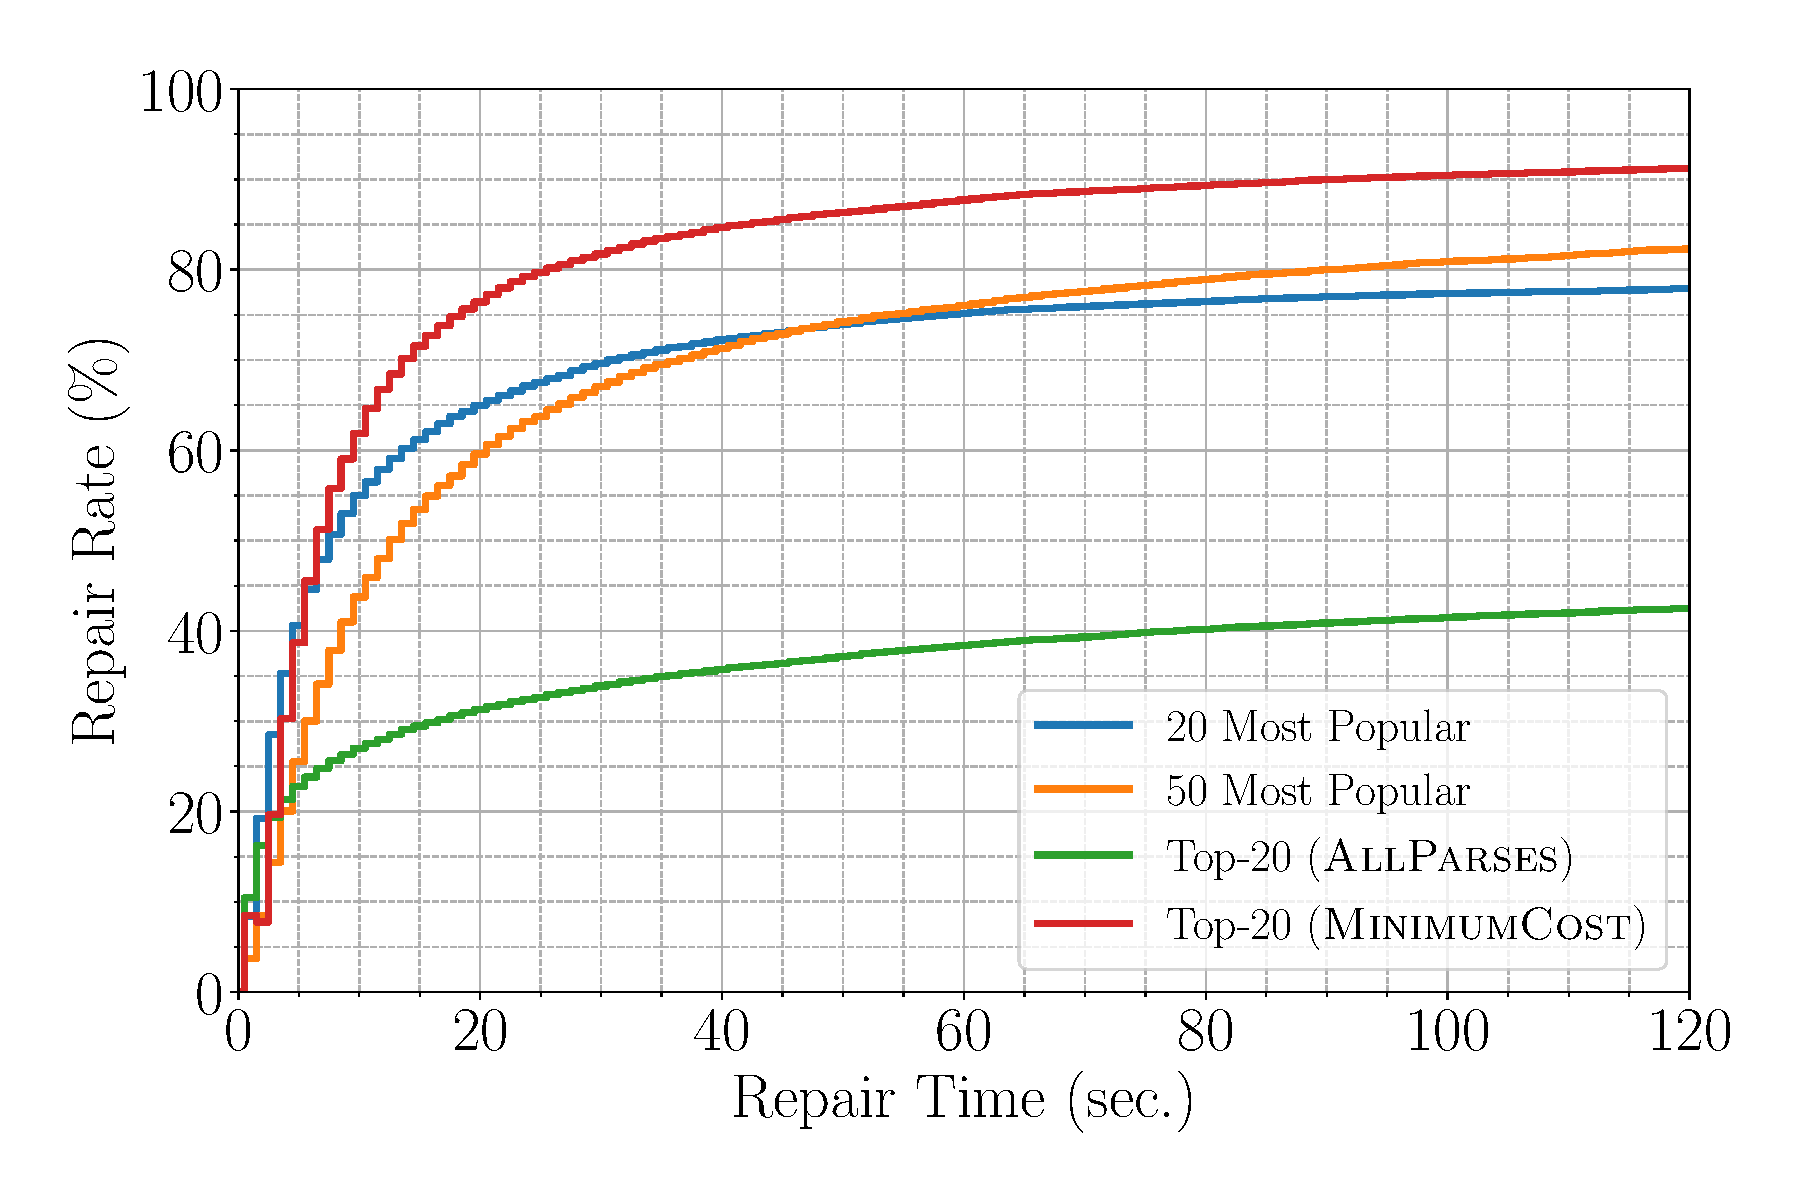
\includegraphics[width=\linewidth]{tool-repair-rate.pdf}
    \caption{The repair rate for all the approaches in
    \autoref{tab:seq2parse_full_results}}
    \label{fig:tool-repair-rate}
  \end{minipage}
\end{figure}

\subsection{RQ3: Efficiency}
\label{sec:eval:efficiency}

% \begin{figure}[t]
%   \centering
%   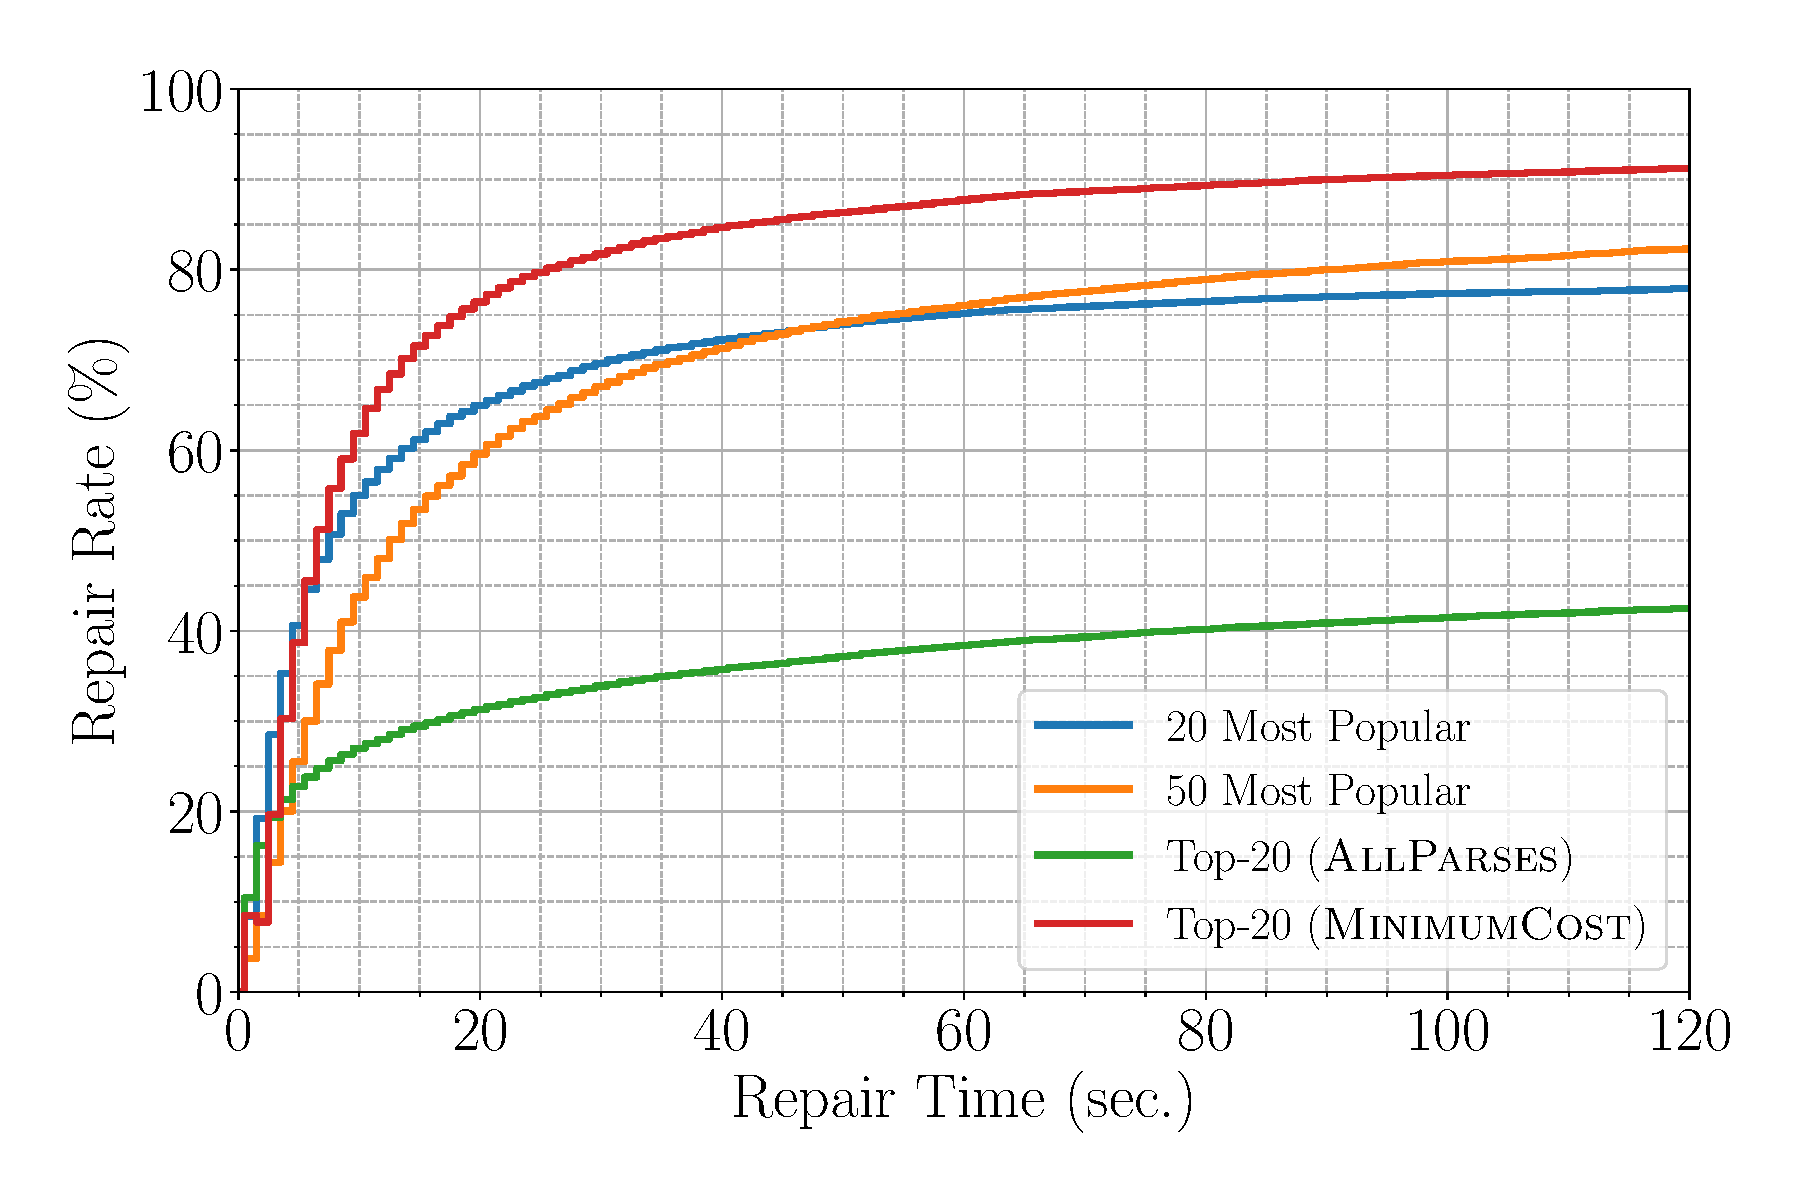
\includegraphics[width=0.8\linewidth]{tool-repair-rate.pdf}
%   \caption{The repair rate for all the approaches in
%   \autoref{tab:seq2parse_full_results}}
%   \label{fig:tool-repair-rate}
% \end{figure}

Next we evaluate \toolname's efficiency by measuring how many programs it is
able to parse. We limit each ECE-Parser to 5 minutes. (In general the procedure
is undecidable, and we conjecture that a longer timeout will diminish the
practical usability for novices.) We compare the efficiency of \toolname for all
the versions of \autoref{tab:seq2parse_full_results}.

\autoref{fig:tool-repair-rate} shows the cumulative distribution function of all
\toolname approaches' repair rates over their parse time. We observe that using
the top 20 error production rule predictions is the most efficient while
maintaining the highest parse accuracy at all times, with a repair rate of
78.10\% within 20 seconds and a median parse time of 5.3 seconds.

We observe that, using a fixed set of the 20 and 50 most popular rules for
\toolname to parse programs with syntax errors, a 61.41\% and 65.20\%
respectively within 20 seconds, and median parse times of 7.0 and 10.1 seconds
respectively. The 50 most popular ECE-Parser is parses less programs until the
45 seconds but the extra number of error rules aids the ECE-Parser to parse more
after that point and outperform the 20 most popular ECE-Parser.

We also observe that \toolname successfully parses around 38.50\% of the
programs with its \textsc{AllParses} approach in 20 seconds and has a median
parse time of 23.2 seconds. While this approach is much less efficient that the
others. due to the vast amount of states is keeps internally in its data
structure, it is also able to generate the exact human repair in 1 out of 3
times which makes still a very valuable approach (\S~\ref{sec:eval:precise}).

\begin{framed}
  \noindent \toolname can parse programs with syntax errors for the vast
  majority of the test set in under 20 seconds.
\end{framed}

\subsection{RQ4: Usefulness}
\label{sec:eval:useful}

We are also interested in the subjective human understanding of the quality
and helpfulness of \toolname's repairs.
This is so because \toolname's primary use case is as an aid for programmers
faced with parse errors. 31\% of repairs produced by \toolname
using its \textsc{AllParses} approach are identical to the historical human repair
and thus likely helpful for programmers. However, it may be that \toolname's fixes
are still helpful for debugging even when they differ from the historical human
repair. To investigate this hypothesis, we conduct a human study of the quality and
debugging helpfulness of \toolname fixes.

\mypara{Human Study Setup.} We recruited participants from two large public
research institutions (names omitted for blind-review) and through Twitter.
The study was online, took around 30 minutes, and participants could enter a
drawing for one of two \$50 awards. In the study, participants
were each asked to rate 15 debugging hints randomly selected from a corpus of 50
stimuli\footnote{All human study stimuli are included in our replication
package at FIXME}.

We created the stimuli by selecting 50 buggy programs from the Python Tutor dataset
for which \toolname and the historical human produced different fixes. Other than
ensuring a wide array of difficulty (as assessed by how long the
human took to fix the error), programs were selected randomly. Each
stimulus consisted of a buggy program, its associated syntax
error, and a potential program fix presented as a \emph{debugging hint}
(see Figure FIXME for an example stimulus).
For each stimulus, we produced two versions: one where the debugging hint was
generated by \toolname and one where the debugging hint was the historical
human-created fix.

Participants rated the quality and helpfulness of each debugging
hint using a 1-5 Likert scale.
They also indicated if the debugging hint provided helpful information beyond
that in the Python error message %\footnote{In this study, we used error messages from Python 3.10. Compared to earlier Python versions, 3.10 includes improved error messages for Syntax Errors.}.
Participants were unaware of if any given
hint was generated by a human or \toolname, and participants were never shown both the
tool-generated and human-generated repairs to the same buggy program. To be included
in analysis, participants had to assess the quality and debugging helpfulness of at
least four stimuli. Overall, we analyze 527 unique stimuli ratings from 39 valid
participants (246 for human-generated foxes and 281 for \toolname fixes).

\mypara{Overall Results.} Humans in our study find that repairs produced by
\toolname are lower in both quality and debugging helpfulness than those produced
by humans (2.9/5 helpfulness for tool-produced repairs vs 3.7/5 for human-produced
repairs, p < 0.001). However, we find that humans still often find \toolname's fixes
helpful for debugging: participants found that \toolname repairs contained helpful
debugging information beyond that contained in the Python Error message 48\% of
the time (134/281). This additional helpful debugging information was often in both
the content (73\% of the time) and location (55\% of the time) of the generated
repair. Additionally, \toolname fixes are helpful for easy and hard Syntax Errors
alike: we found no statistically significant difference between the helpfulness or
quality of \toolname's repairs for easy parse errors (those repaired by the human in under
40 seconds) or hard parse errors (those repaired by the human in over 40 seconds). %p = 0.07 and 0.13 respectively if we have room to include
Overall, these results indicate that even when \toolname repairs differ from
that of the historical human repair, they may still often be helpful for debugging.

\mypara{Individual Stimuli.}

Beyond an analysis of FIXME:TOOL’s overall quality and helpfulness, we also


\begin{framed}
  \noindent
While humans find that \toolname repairs that differ from the historical human repair are
of lower quality than the historical human repair, they still contain helpful
debugging information beyond that in the Python error message 48\% of the time.
Additionally, over half of \toolname fixes (56\%) were either indistinguishable from
or more helpful than those produced by humans.
\end{framed}

\section{Related Work}
\label{sec:related-work}

There is a vast literature on automatically repairing or patching programs:
we focus on the most closely related work on providing feedback for parse
errors.

\mypara{Error-Correcting Parsers}
%
As we have already demonstrated, error-correcting parses have been proposed for
repairing syntax errors and we have extensively described ECE-Parsers
\citep{Aho_1972}. The technique presented by \citet{Burke1987} describes another
EC-Parser, which is applicable with LR and LL parsing. It uses three phases:
first attempts to repair the parse error by symbol insertions, deletions, or
substitutions. If that fails, it tries to close one or more open code blocks and if
that fails, it removes code surrounding the erroneous symbol. Finally, it uses
\emph{deferred parsing} that may be viewed as double parsing, where one main
parser moves forward as much as possible, whereas a second parser is $k$ steps
behind, so that it can backtrack to a state $k$ steps before efficiently if a
phase fails. \citet{VanDerSpek_2005} have shown that the previous approach is not
applicable in real-world languages for some specific cases (\eg multiple
function definitions) and has suggested an improvement that works with the
\textsc{JavaCC} parser generator and a form of \emph{follow-set error recovery}.
\citet{Corchuelo2002} have suggested an error-correcting version of the popular
LR parser. Rather than focusing on error production rules, this method adds
\emph{error-repair transitions} along with the regular shift/reduce operations.
It employs a simple cost model and heuristics to limit the explosion of the
repair search space. Finally, \citet{Thompson1976} has suggested using
\emph{probabilistic parsing} to overcome the drawback of selecting the
minimal-edit repair by using a PCFG to select the most \emph{probable} repair
parse. However, these approaches are impractical and inefficient for real-world
applications, as they can only successfully parse small examples or use tiny
grammars. In contrast, \toolname relies on pre-trained sequence models to
efficiently explore the repair search space for a minimal overhead in real-time
parsing.

\mypara{Sequence Models in Software Engineering}
%
\citet{Rahmani2021} and \citet{Verbruggen2021} have suggested using pre-trained
auto-regressive transformer models, such as \textsc{GPT-3} \citep{GPT2020}, to
augment pre-existing program synthesis techniques. They use pre-trained models
to acquire semantic power over smaller subproblems that can't be solved with the
syntactic power of classic program synthesis. Similar to \toolname, their work
uses established pre-existing algorithms from the NLP and PL research areas.
However, \toolname trains its own Transformer-based model to augment an
error-correcting parsing algorithm, providing more focused prior knowledge than
a pre-trained sequence model, thus making our model highly accurate.

\mypara{Sequence Models for Parsing}
%
\textsc{SynFix} \citep{Bhatia2016} and \emph{sk\_p} \citep{Pu2016} are two
systems that use seq2seq models consisting of Long Short-Term Memory networks
(LSTMs). They mostly focus on educational programming tasks in order to learn
task-specific patterns for fixing erroneous task solutions. \textsc{SynFix} uses
a model per task and uses as an input sequence the program prefix until the
error locations that the language parser provides. \emph{sk\_p} (while it does
not solely focus on syntax errors) makes sequence predictions per program line,
by considering only the abstracted context lines (previous and next lines). The
model is applied to every program line and the predictions with the highest
probabilities are selected. \toolname manages to parse and repair a large number
of programs regardless the task they are trying to solve by encoding the full
erroneous programs with a state-of-the-art Transformer model and utilizing an
EC-Parser to parse them accordingly, thus achieving a much higher accuracy.
Additionally, it uses a real-world dataset of millions of \python programs to
learn to effectively parse programs, while \textsc{SynFix} and \emph{sk\_p} are
trained on smaller datasets of correct programs that have errors manually
introduced on training, possibly skewing the predictions away from real-world
fixes.

\textsc{DeepFix} \citep{Gupta2017} is another seq2seq approach for repairing
syntactical errors in \textsc{C} programs. It relies on stacked \emph{gated
recurrent units} (GRUs) with attention and applies some simple abstraction over
the terminal tokens. The input programs are broken into subsequences for each
line and the model gets as input all the line subsequences with their associated
line numbers. \textsc{DeepFix} only predicts single line fixes and its predictions
are applied iteratively multiple times, if multiple parse errors exist or until
the parse error is fixed. \textsc{DeepFix} struggles with the same problems as
previous work, as it solely relies on the sequence models' capability to learn
the full grammar and repair programs with minimal abstraction and prior
knowledge over the language.

\emph{Lenient parsing} \citep{Ahmed_2021} presents another sequence model
approach. It uses \emph{two seq2seq Transformer models} and trains them with a
large corpus of code. One model is trained to repair and create proper nested
blocks of code, called \textsc{BlockFix}, and the second one, called
\textsc{FragFix}, repairs and parses fragments of code (\eg program statements)
within a repaired block. \textsc{BlockFix} tokenizes input program block in a
similar manner to our abstracted token sequences, by abstracting identifiers,
constants, expressions, etc., and is trained on pairs of valid and
manually-corrupted blocks. On the other hand, \textsc{FragFix} repairs on a
program-statement level within blocks (mostly focusing on missing semicolons and
commas), by using serialized versions of ASTs and error hints manually injected
on the ASTs. While this overall approach is mostly automatic, it relies on the
manual corruption of a dataset to generate erroneous programs that may not
correlate to the errors actual developers make and solely relies on the seq2seq
models to learn the underlying language model and make repairs. In contrast,
\toolname mitigates this problem by learning how programmers fixed programs from
a large corpus and by abstracting via partial parses. Additionally, our use of
EC-Parsers and the language grammar significantly improves program repairs.

\mypara{Graph models for parsing}
%
Graph-based Grammar Fix (\textsc{GGF}) \citep{Wu2020} suggested using a
\emph{Gated Graph Neural Network} encoder for the partial parse trees that can
be acquired from a LALR parser and a \emph{GRU} encoder for the parts of the
program sequence that are not parsed. This approach aims to better summarize the
context of the program in order to train more accurate models. Its models then
predict an error location in the program sequence and a token suggestion for the
repair. This single-token repair approach is applied iteratively multiple times
until the program correctly parses. While this approach is much more accurate
than any previous work, as it repairs \emph{58\%} of the syntax errors of a
real-world dataset, it still lacks the advantages of using a parser with the
actual grammar as the final step of the repairing process that \toolname takes
benefit from and relies again on the model to learn the semantics of the
language.

\mypara{Neural Machine Translation (NMT) for Program Repair}
%
\textsc{CoCoNuT} \citep{Lutellier2020} proposed a complex architecture that uses
a new \emph{context-aware NMT model} that has two separate \emph{Convolutional
Neural Network (CNN)} encoders, one for the buggy lines and one for their
surrounding lines. It also uses \emph{ensemble learning} to train NMT models of
different hyper-parameters to capture different relations between erroneous and
correct code. This approach uses a minimal level of abstraction over the input
programs, with only a subword-level tokenization to minimize the vocabulary size
and make training tractable.
%
\textsc{CURE}~\citep{Jiang_2021} suggested a similar \emph{code-aware NMT model}
that is pre-trained using unsupervised learning on correct programs. It also
uses a programming language \textsc{GPT} \citep{GPT2020} model that learns to
predict the next token in program sequences and uses beam search to maintain a
small set of accurate repairs.

\GS{TODO: We had this part in rebuttal: "we will expand Section 8 with
qualitative comparisons to the prominent CoCoNut, as well as the Facebook
TransCoder paper (which uses tests rather than a metric like BLEU). In
particular, while being careful to indicate that it would be an
apples-to-oranges comparison, we can provide readers with additional context by
reporting some of the success rates from those approaches (such as the 509/4456
for CoCoNut on large standard software defects) and indicating which of those
successes are likely to translate to this domain and which are not. We will add
clarity to that discussion by following R1’s suggestion that we indicate which
algorithmic aspects of our approach represent progress over such
state-of-the-art techniques (e.g., our novelty lies in applying neural and
symbolic approaches in tandem, while error correcting parsing is already
well-established)".}
% \section{Conclusion}
\label{sec:conclusion}

We have presented \emph{neurosymbolic parse program repair}, a new neurosymbolic
approach to automatically repair parse errors.
%
Our approach is to use a dataset of ill-parsed programs and their fixed versions
to train a Transformer classifier (neural component) which allows us to
accurately predict EC-rules for new programs with syntax errors. In order to
make accurate predictions, we abstract the low-level program token sequences
using partial parses and probabilistic grammars. A small set of predicted
EC-rules is finally used with an ECE-Parser (symbolic component) to parse and
repair new ill-parsed programs in a tractable and precise manner.

We have implemented our approach in \toolname, and demonstrated, using a corpus
of 1,100,000 ill-parsed \python programs drawn from two years of data from an
online web-based educational compiler, that \toolname makes accurate EC-rule
predictions 81\% of the time when considering the top 20 EC-rules, and that the
predicted EC-rules let us parse and repair over 94\% of the test set in 2.1 sec
median parse time, while generating the user fix in almost 1 out of 3 cases.
%
Finally, we conducted a user study with 39 participants which showed that
\toolname's edit locations and repairs are useful and helpful, even when they
are not equivalent to the user's fix.



%% Acknowledgments
\begin{acks}                            %% acks environment is optional
                                        %% contents suppressed with 'anonymous'
  %% Commands \grantsponsor{<sponsorID>}{<name>}{<url>} and
  %% \grantnum[<url>]{<sponsorID>}{<number>} should be used to
  %% acknowledge financial support and will be used by metadata
  %% extraction tools.
  This material is based upon work supported by the
  \grantsponsor{GS100000001}{National Science
    Foundation}{http://dx.doi.org/10.13039/100000001} under Grant
  No.~\grantnum{GS100000001}{nnnnnnn} and Grant
  No.~\grantnum{GS100000001}{mmmmmmm}.  Any opinions, findings, and
  conclusions or recommendations expressed in this material are those
  of the author and do not necessarily reflect the views of the
  National Science Foundation.
\end{acks}


%% Bibliography
\bibliography{bibliography}


%% Appendix
% \appendix
% \section{Appendix}

% Text of appendix \ldots

\end{document}
